% Emerald Publishing - Construction Innovation Submission Template
% by Oleksandr Melnyk
% Ver 0.0.4
% Based on: https://www.emeraldgrouppublishing.com/journal/ci#author-guidelines


\documentclass[12pt]{article}
\usepackage{setspace}
\onehalfspacing
\usepackage[english]{babel}
\usepackage{appendix}
\usepackage{tikz}
\usetikzlibrary{patterns}
\usepackage{standalone}

% Set page size and margins
% Replace `letterpaper' with `a4paper' for UK/EU standard size
\usepackage[a4paper,top=2cm,bottom=2cm,left=3cm,right=3cm,marginparwidth=1.75cm]{geometry}

\usepackage{sectsty}
\sectionfont{\fontsize{15}{15}\selectfont}

% Useful packages
\usepackage{amssymb,amsmath}
\usepackage{amsthm}
\newtheorem{theorem}{Theorem}
\newtheorem{proposition}{Proposition}
\newtheorem{lemma}{Lemma}
\newtheorem{corollary}{Corollary}
\newtheorem{remark}{Remark}
\usepackage{siunitx}
\PassOptionsToPackage{hyphens}{url}\usepackage{hyperref}
\usepackage{cleveref}
\usepackage[utf8]{inputenc}
\usepackage[left]{lineno}
\usepackage{csquotes}
\usepackage{booktabs}
\usepackage{longtable}
\usepackage{adjustbox}
\usepackage{array}
\usepackage{url}
\usepackage{titlesec}
%\usepackage[compatibility=false]{caption}
\usepackage{authblk}
\usepackage{xcolor} % Load the xcolor package for color options
\renewcommand{\thetable}{\Roman{table}}

% Define a new format for \subsection
\titleformat{\subsection}
  {\mdseries\itshape\large} % Medium series, italic shape, and large font size
  {\thesubsection}{1em}{} % Numbering, spacing, and the section title itself


% Emerald Harvard Citation Style

\usepackage[style=authoryear,backend=biber,natbib=true,maxcitenames=2,uniquelist=false,url=true,doi=false,eprint=false,isbn=false]{biblatex}
\addbibresource{refer.bib} % your .bib file
\addbibresource{AI.bib} % your .bib file

% Customizing biblatex for Harvard style
% Customizing biblatex for Harvard style
\DeclareNameAlias{sortname}{family-given}
\DeclareNameAlias{default}{family-given}

\renewbibmacro{in:}{}
\DeclareFieldFormat[article]{title}{\mkbibquote{#1}\addcomma}
\DeclareFieldFormat[book]{title}{\mkbibemph{#1}\addcomma}
\DeclareFieldFormat[bookinbook]{title}{\mkbibemph{#1}\addcomma}
\DeclareFieldFormat[inbook]{title}{\mkbibquote{#1}\addcomma}
\DeclareFieldFormat[incollection]{title}{\mkbibquote{#1}\addcomma}
\DeclareFieldFormat[inproceedings]{title}{\mkbibquote{#1}\addcomma}
\DeclareFieldFormat[manual]{title}{\mkbibemph{#1}\addcomma}
\DeclareFieldFormat[misc]{title}{\mkbibemph{#1}\addcomma}
\DeclareFieldFormat[thesis]{title}{\mkbibemph{#1}\addcomma}
\DeclareFieldFormat[unpublished]{title}{\mkbibquote{#1}\addcomma}
\DeclareFieldFormat[patent]{title}{\mkbibemph{#1}\addcomma}
\DeclareFieldFormat[report]{title}{\mkbibemph{#1}\addcomma}
\DeclareFieldFormat[online]{title}{\mkbibquote{#1}\addcomma}
\DeclareFieldFormat[software]{title}{\mkbibemph{#1}\addcomma}
\DeclareFieldFormat[booklet]{title}{\mkbibemph{#1}\addcomma}
\DeclareFieldFormat[periodical]{title}{\mkbibemph{#1}\addcomma}
\DeclareFieldFormat[standard]{title}{\mkbibemph{#1}\addcomma}

\DeclareFieldFormat[article]{journaltitle}{\iffieldundef{shortjournal}{\mkbibemph{#1}\addcomma}{\mkbibemph{\printfield{shortjournal}}\addcomma}}
\DeclareFieldFormat{volume}{\bibstring{volume}~#1}
\DeclareFieldFormat{number}{\bibstring{number}~#1}

% Definitions for "Vol." and "No."
\DefineBibliographyStrings{english}{
  volume = {Vol.},
  number = {No.}
}

\renewbibmacro*{volume+number+eid}{%
  \printfield{volume}%
  \setunit*{\addspace}%
  \printfield{number}%
  \setunit{\addcomma\space}%
  \printfield{eid}}

\renewbibmacro*{journal+issuetitle}{%
  \usebibmacro{journal}%
  \setunit*{\addcomma\space}%
  \usebibmacro{volume+number+eid}%
  \setunit{\addcomma\space}%
  \usebibmacro{issue+date}}

\renewbibmacro*{publisher+location+date}{%
  \printlist{publisher}%
  \iflistundef{location}
    {\setunit*{\addcomma\space}}
    {\setunit*{\addcolon\space}}%
  \printlist{location}%
  \setunit*{\addcomma\space}%
  \usebibmacro{date}}

\renewcommand*{\bibpagespunct}{\addcomma\space}

\newcommand\YL[1]{\textcolor{blue}{YL: #1}}	

% Customizing page field format to prevent duplication
% \DeclareFieldFormat{pages}{%
%   \mkfirstpage[{\mkpageprefix[page]{#1}}]{#1}}

% Customizing citations for Harvard style
\DeclareCiteCommand{\cite}[\mkbibparens]
  {\usebibmacro{prenote}}
  {\usebibmacro{citeindex}%
   \usebibmacro{cite}}
  {\multicitedelim}
  {\usebibmacro{postnote}}

\renewbibmacro*{cite:labelyear+extrayear}{%
  \iffieldundef{labelyear}
    {}
    {\printtext[bibhyperref]{%
       \printfield{labelyear}%
       \printfield{extrayear}}}}

\renewbibmacro*{cite:labeldate+extradate}{%
  \iffieldundef{labelyear}
    {}
    {\printtext[bibhyperref]{%
       \printfield{labelyear}%
       \printfield{extradate}}}}

\AtEveryBibitem{
  \clearfield{month}
  \clearfield{day}
  \ifentrytype{book}{
    \clearlist{location}
  }{}
}

% Formatting "et al." in italics followed by a comma
\DefineBibliographyStrings{english}{
  andothers = {\textit{et al.},}
}

\DeclareFieldFormat[article]{volume}{\bibstring{jourvol}\addnbspace #1}
\DeclareFieldFormat[article]{number}{\bibstring{number}\addnbspace #1}
\DeclareFieldFormat[article]{volume}{Vol. #1}
\DeclareFieldFormat[article]{number}{No. #1}
% Customizing DOI field format to lowercase "doi"
%\DeclareFieldFormat{doi}{\bibstring{doi}\addcolon\space\url{#1}}

% % Customizing URL field format to "available at:"
% \DeclareFieldFormat{url}{\bibstring{available at}\addcolon\space\url{#1}}
% \DeclareFieldFormat{urldate}{\mkbibparens{accessed \addspace#1}}

% % Customizing urldate to match the required format
% \DeclareFieldFormat{urldate}{%
%   \mkbibparens{accessed\space%
%     \thefield{urlday}\addspace%
%     \mkbibmonth{\thefield{urlmonth}}\addspace%
%     \thefield{urlyear}}}


% Configure cleveref
%\crefformat{figure}{#2Figure~#1#3}
%\Crefformat{figure}{#2Figure~#1#3}
%\crefformat{table}{#2Table~#1#3}
%\Crefformat{table}{#2Table~#1#3}
\crefformat{section}{#2Section~#1#3}
\Crefformat{section}{#2Section~#1#3}

%Front Matter
\author[1]{Yang K. Lu}
\author[2]{Eunseong Ma}

\affil[1]{HKUST}
\affil[2]{Yonsei}

%\title{\Large Anticipating AI-Driven Skill Demand: Human Capital Responses and Macro-Level Implications}
\title{\LARGE AI and Human Capital Accumulation: \\ Aggregate and Distributional Implications\footnote{Author emails: yanglu@ust.hk; masilver@yonsei.ac.kr}}


\begin{document}
\maketitle


\begin{abstract}
This paper develops a model to analyze the effects of AI advancements on human capital investment and their impact on aggregate and distributional outcomes in the economy. We construct an incomplete markets economy with endogenous asset accumulation and general equilibrium, where households decide on human capital investment and labor supply. Anticipating near-term AI advancements that will alter skill premiums, we analyze the transition dynamics toward a new steady state. Our findings reveal that human capital responses to AI amplify its positive effects on aggregate output and consumption, mitigate the AI-induced rise in precautionary savings, and stabilize the adjustments in wages and asset returns. Furthermore, while AI-driven human capital adjustments increase inequalities in income, earnings, and consumption, they unexpectedly reduce wealth inequality.\\
\\
%add 6 keywords
\textbf{Keywords:} AI, Job Polarization, Human Capital, Inequality
\end{abstract}
\linenumbers

\newpage

\section{Introduction}
\label{sec:introduction}

A defining feature of recent AI advancements is their ability to perform complex, cognitive, non-routine tasks -- capacities that once required substantial education and expertise. This fundamental difference sets AI apart from earlier waves of automation or computerization, which primarily replaced manual or routine labor.\footnote{For example, AI tools in medical diagnostics now assist radiologists in analyzing medical images, potentially reducing demand for entry-level radiologists while simultaneously increasing the productivity of senior professionals.} In this paper, we make a central assumption -- supported by a growing body of evidence -- that AI adoption reduces the premium for middle-level skills while increasing the value of high-level expertise. Based on this assumption, we develop a model to study the effects of AI advancements on human capital investment and their subsequent impact on aggregate and distributional outcomes of the economy.

Recent labor market data highlight the disproportionate impact of AI on entry-level employment opportunities. Bloomberg \cite{bloomberg2025} reports that, in the words of Matt Sigelman, president of the Burning Glass Institute, ``Demand for junior hires in many college-level roles is already declining, even as demand for experienced hires in the same jobs is on the rise.'' According to Revelio Labs \cite{reveliolabs2025}, postings for entry-level jobs in the US declined by about 35\% since January 2023, with roles more exposed to AI experiencing even steeper reductions. 

Recent experimental evidence reviewed by \citet{calvino_effects_2025} shows that workers' productivity gains from AI depend on their skill levels and experience. On simpler tasks where AI performs well, the technology can narrow the productivity gap between experienced and less experienced workers. However, for more complex tasks that AI cannot yet perform effectively, those with greater digital proficiency or task-specific experience achieve higher productivity gains, as successful use of AI in these settings requires more advanced skills and experience that involves understanding AI's capabilities and limitations.

Firm-level evidence reveals similar patterns. \citet{aghion2019} documents that the average worker in low-skilled occupations receives a significant wage premium when employed by a more innovative firm. \citet{de_souza_artificial_2025} finds that the adoption of AI in Brazilian firms increases employment for low-skilled production workers but reduces employment and wages for middle-wage office workers. \citet{asam_generative_2025} report that GitHub Copilot enables software startups to raise initial funding 19\% faster with 20\% fewer developers, and that these productivity gains disproportionately benefit startups with more experienced founders.

In anticipation of these changes, households are likely to adjust their human capital investments.
A 2022 report by Higher Education Strategy Associates finds that following decades of growth, dropping student enrollment in higher education has become a major trend in the Global North \cite{hesa2022}. In the U.S., the public across the political spectrum has increasingly lost confidence in the economic benefits of a college degree.\footnote{Pew Research Center reports that about half of Americans say having a college degree is less important today than it was 20 years ago in a survey conducted in 2023 \cite{pew2024}. A 2022 study from Public Agenda \cite{publicagenda2022}, a nonpartisan research organization, shows that young Americans without college degrees are most skeptical about the value of higher education.} 

On the other hand, demand for sector-based training and reskilling opportunities has been rising. The Oliver Wyman Forum's 2024 study \cite{oliwyman2024} documents widespread and significant gaps between employees’ desire for reskilling in generative AI and the opportunities their employers are willing to offer. The study estimates that, over the coming decade, billions of workers will need upskilling and millions may require complete reskilling.


This paper constructs an incomplete markets economy with endogenous asset accumulation and general equilibrium to study how AI's effects on skill premia interact with households' human capital investment, and their subsequent impact on aggregate and distributional outcomes of the economy.


We consider an economy with three sectors, each requiring low, middle, or high levels of skill (human capital) and exhibiting increasing labor productivity. Households can invest in human capital to move up to more productive sectors; without such investment, their skills depreciate, causing them to shift toward less productive sectors over time. Human capital investment occurs at two levels: a basic level achievable while working, and a higher level that demands full-time commitment, such as pursuing higher education or reskilling training. Households face uninsurable idiosyncratic productivity shocks, affecting both their labor productivity and the returns to human capital investment.

We model AI advancements as increasing the productivity for the low and high sectors but not for the middle sector so that the skill premium of the middle sector decreases and the skill premium of the high sector increases. 

Using a two-period partial equilibrium model, we show that the effects of AI on skill premia discourage human capital investment for households in the low sector and encourage human capital investment for households in the middle sector, thereby increasing human capital inequality. 

Human capital investment via full-timing training crowds out households' labor supply so that households in the low sector supplies more labor whereas households in the high sector supplies less labor, in response to the AI advancements. 

We also investigate the interaction between human capital investment and saving. When households could adjust their human capital, the skill premium matters for their idiosyncratic risk exposure because when they move across sectors, their labor income is affected by the skill premium. As AI reduces the skill premium of the middle sector, households in the low sector has lower idiosyncratic risk exposure and thus reduce their saving. Conversely, AI increases the skill premium of the high sector, households in the high sector has higher idiosyncratic risk exposure and thus increase their saving. AI's effect on saving of the middle-sector households is ambiguous.

At the economy level, the effects of AI advancements depend on the sectoral redistribution of households and the general equilibrium effects via wage and capital return responses. We quantify these effects using a fully-fledged dynamic quantitative model that incorporates an infinite horizon, endogenous asset accumulation, and general equilibrium. The model is calibrated to reflect key features of the U.S. economy, capturing realistic household heterogeneity. The steady state distribution of human capital without AI advancements pins down the sectoral distribution of households. We then introduce fully anticipated AI advancements happening in the near future and study the transition dynamics from the current state of the economy to the eventual new steady state. 

We find that aggregate human capital rises sharply even before AI introduction, indicating that a substantial portion of workers, anticipating changes in skill premium, leave the labor force early to accumulate human capital. The economy also experiences AI-induced job polarization, with a notable reallocation of workers from the middle sector to either low or high sectors.

Building on these labor dynamics, our model examines how AI influences both the aggregate and distributional outcomes of the economy. Our focus is on how human capital adjustments reshape AI’s effects on each of these outcomes by contrasting transition dynamics between the benchmark model and a model with human capital fixed at the initial steady state.

Our findings reveal that human capital responses to AI amplify its positive effects on aggregate output and consumption, mitigate the AI-induced rise in precautionary savings, and stabilize the adjustments in wages and asset returns. Furthermore, while AI-driven human capital adjustments increase inequalities in income, earnings, and consumption, they unexpectedly reduce wealth inequality. We also show that the redistribution channel is the dominant factor in the effects of human capital adjustments, whereas the general equilibrium channel, via wage and capital return changes, plays a comparatively minor role.

%Suppose that labor supply declines as a result of households in the middle sector exiting the workforce to invest in their human capital in anticipating the AI advancements. The equilibrium wage will increase, disproportionately benefiting high-sector workers whose labor produces more effective units. This will encourage further shifts from the middle sector and amplifying human capital adjustments.

INTRODUCING PRECAUTIONARY SAVING MOTIVE IN THE WAGE POLARIZATION INVESTIGATION \citet{autor_polarization_2006}\citet{Autor2013}

\subsection{Related Literature}
This paper relates to the literature examining how technological advancements,
including AI, have significantly contributed to job polarization.
\citet{Goos2007} show that since 1975, the United Kingdom has experienced
job polarization, with increasing employment shares in both high-
and low-wage occupations. \citet{Autor2013} expanded on this by providing
a unified analysis of the growth of low-skill service occupations,
highlighting key factors that amplify polarization in the U.S. labor
market. Empirical evidence from \citet{Goos2014} further confirms
pervasive job polarization across 16 advanced Western European economies.
In the U.S., \citet{Acemoglu2020} show that robots can reduce employment
and wages, finding robust negative effects of automation on both in
various commuting zones.

The introduction of AI and robotics has had adverse effects on labor
markets, with significant implications for employment and labor force
participation. \citet{Lerch2021} highlights that the increasing use
of robots not only displaces workers but also negatively impacts overall
labor force participation rates. Similarly, \citet{Faber2022} demonstrate
that the detrimental effects of robots on the labor market have resulted
in a decline in job opportunities, particularly in sectors where automation
is prevalent. These findings suggest that while technological advancements
bring productivity gains, they simultaneously reduce employment prospects
and participation in the labor market, exacerbating economic challenges
for certain groups of workers.

The introduction of AI and robotics also influences human capital
accumulation as workers respond to technological disruption. Faced
with the employment risks brought about by automation, many exposed
workers may invest in additional education as a form of self-insurance,
rather than relying on increases in the college wage premium \parencites{Atkin2016,Beaudry2016}. Empirical evidence supports this response.
\citet{DiGiacomo2023} find that for every additional robot adopted
in U.S. local labor markets between 1993 and 2007, four individuals
enrolled in college, particularly in community colleges, indicating
a rise in educational investments triggered by automation. Similarly,
\citet{Dauth2021} show that within German firms, robot adoption has
led to an increase in the share of college-educated workers, as firms
prioritize higher-skilled employees over those with apprenticeships. 

The response of human capital accumulation to technological disruption could also go to the other extreme. 


The rise of AI and automation also plays a significant role in exacerbating
general inequality, particularly through its impact on education and
wealth distribution. \citet{Prettner2020} present a model showing
that innovation-driven growth leads to an increasing proportion of
college graduates, which in turn drives higher income and wealth inequality.
As technology advances, workers with higher educational attainment
benefit disproportionately, widening the gap between those with and
without advanced skills. \citet{Sachs2012} also explore this dynamic,
providing a model within an overlapping generations framework that
examines the interaction between automation and education. They demonstrate
how automation can further entrench inequality by favoring workers
with higher levels of education, as those without adequate skills
are more likely to be displaced or see their wages stagnate. This
interaction between technological change and educational attainment
not only amplifies economic inequality but also perpetuates disparities
in wealth across generations.

The rest of the paper is organized as follows. Section 2 describes the model environment. Section 3 solves the household's problem using a two-period version of the model. Section 4 solves the fully-fledged quantitative model and calibrates it to fit key features of the U.S. economy, including employment rate, human capital investment, and household heterogeneity. Section 5 incorporates AI into the quantitative model and examines its economic impact on both aggregate and distributional outcomes. Section 6 analyzes how human capital adjustments change the economic impact of AI advancements. Section 7 concludes.

\section{Model Environment }
\label{sec:model}
Time is discrete and infinite. 
There is a continuum of households. Each household is endowed with one unit of indivisible labor and faces idiosyncratic productivity shock, $z$, that follows an AR(1) process in logs:
\begin{equation}
    \label{eq:z}
\ln z'=\rho_z\ln z + \varepsilon_z, \varepsilon_z \overset{\mathrm{iid}}{\sim} N(0,\sigma_z^2)
\end{equation}
The asset market is incomplete following \citet{aiyagari_uninsured_1994}, and the physical capital, $a$, is the only asset available to households to insure against this idiosyncratic risk. Households can also invest in human capital, $h$, which allows them to work in sectors with different human capital requirement.

\subsection{Production Technology}
The production technology in the economy is a constant-returns-to-scale Cobb-Douglas production function:
\begin{equation}
    F(K,L)=K^{1-\alpha} L^{\alpha}
\end{equation}
$K$ represents the total physical capital accumulated by households, while $L$ denotes the total effective labor supplied by households, aggregated across three sectors: low, middle, and high. The marginal products of capital and effective labor determine the economy-wide wage rate, $w$, and interest rate, $r$.

These sectors differ in their technologies for converting labor into effective labor units and in the levels of human capital required for employment. 
The middle sector employs households with human capital above $h_M$ and converts one unit of labor to one effective labor unit. The high sector, requiring human capital above $h_H$, converts one unit of labor to $1+\lambda$ effective units, while the low sector, with no human capital requirement, converts one unit into $1-\lambda$ effective units. This implies a sectoral labor productivity $x(h)$ that is a step function in human capital:
\begin{equation}
    \label{eq:x}
x(h)=\left \{ 
\begin{array}{cl}
1-\lambda  & \text{low sector if }h<h_{M} \\ 
1 & \text{middle sector if }h_{M}<h<h_{H} \\ 
1+\lambda  & \text{high sector if }h>h_{H}%
\end{array}%
\right. 
\end{equation}
A household $i$ who decides to work thus contributes $z_ix(h_i)$ units of effective labor, where $z_i$ is his idiosyncratic productivity. Denote $n_i \in \{0,1\}$ as the indicator that takes one if the household works and zero if the household does not. The aggregate labor is
\begin{equation}
    L=\int n_iz_ix(h_i)di,
\end{equation}
assuming perfect substitutability of effective labor across the three sectors.

\subsection{Household's Problem}
Households derive utility from consumption, incur disutility from labor and effort of human capital investment. 
A household maximizes the expected lifetime utility by optimally choosing consumption, saving, labor supply and human capital investment each period, based on his idiosyncratic productivity shock $z_t$:
\begin{equation}
\max_{\left \{ c_t,a_{t+1},n_t,e_t\right \}_{t=0}^{\infty }}E_0\left[
\sum\limits_{t=0}^{\infty }\beta^t( \ln c_t-\chi_n n_t-\chi_e e_t ) \right] 
\end{equation}
where $c_t$ represents consumption, $a_{t+1}$ represents saving, $n_t \in \{0,1\}$ is labor supply, and $e_t$ is the effort of human capital investment.

If a household decides to work in period $t$, he will be employed into the appropriate sector according to his human capital $h_t$ and receive labor income $w_tz_tx(h_t)$. The household's budget constraint is
\begin{align}
    c_t+a_{t+1}&=n_t( w_tz_tx(h_t))+(1+r_t)a_t \\
    c_t& \geq 0 \text{ and } a_{t+1} \geq 0
\end{align}
We prohibit households from borrowing $a_{t+1} \geq 0$ to simplify analysis.\footnote{According to \citet{aiyagari_uninsured_1994}, a borrowing constraint is necessarily implied by present value budget balance and nonnegativity of consumption. Since the borrowing limit is not essential to our analysis, we set it to zero for simplicity.} 

Human capital investment can take three levels of effort: $\{0,e_L,e_H\}$. A non-working household is free to choose any of the three effort levels but a working household cannot devote the highest level of effort $e_H$, reflecting a trade-off between working and human capital investment. Hence:
\begin{equation}
e_t \in \{0, e_L, (1-n_t)e_H\}.
\end{equation}
Its contribution to next-period human capital is subject to the productivity shock:
\begin{equation}
h_{t+1}=z_te_t + (1-\delta)h_t
\end{equation}
where $\delta$ is human capital's depreciation rate. 
 
\section{Household Decisions in a Two-Period Model}
In this section, we solve the household's problem with two periods to gain intuition. 


\paragraph{Period-2 decisions}\label{sec:period2}
Households do not invest in human capital or physical capital in the last period. The only relevant decision is whether to work. 

The household works $n=1$ if and only if $z\geq\overline{z}(h,a)$, with $\overline{z}(h,a) $ defined as 
\begin{equation}
    \ln(w\overline{z}(h,a)x(h)+(1+r)a)-\chi_n = \ln((1+r)a)
\end{equation}
The household faces a trade-off between earning labor income and incurring the disutility of working. 
Given the sector-specific productivity $x(h)$ specified in (\ref{eq:x}), the threshold for idiosyncratic productivity, $\overline{z}(h,a)$, takes on three possible values:
\begin{align}
    \label{eq:z-period2}
\overline{z}(h,a)&=\left \{ 
\begin{array}{cl}
\overline{z}(a)\frac{1}{1-\lambda}  & \text{if }h<h_{M} \\ 
\overline{z}(a) & \text{if }h_{M} \leq h<h_{H} \\ 
\overline{z}(a)\frac{1}{1+\lambda}   & \text{if }h>h_{H}%
\end{array}%
\right. \\
\text{where }\overline{z}(a)&:=\frac{(\exp(\chi_n)-1)(1+r)a}{w}
\end{align}
Households with higher human capital is more likely to work, whereas households with higher physical capital is less likely to work. 

\paragraph{Period-1 decisions}\label{sec:period1}
In addition to labor supply, period-1 decisions include saving and human capital investment, both of which are forward-looking and affected by the idiosyncratic risk associated with the productivity shock $z'$. 
Our model also features a trade-off between human capital investment and labor supply as a working household cannot devote the highest level of effort $e_H$ in human capital investment. Therefore, human capital investment grants households the possibility of a discrete wage hike in the future but may entail a wage loss in the current period. 

To see the implication of this trade-off and how it interacts with uninsured idiosyncratic risk, we proceed in two steps. We first derive the period-1 decisions without uncertainty by assuming that $z'$ is known to the household at period 1 and $z'$ is such that the household will work in period 2. We then reintroduce uncertainty in $z'$ and compare the decision rules with the case without uncertainty.


\subsection{Period-1 Labor Supply and Human Capital Investment} 
\subsubsection{Consumption and saving without uncertainty}

The additive separability of household's utility implies that labor supply $n$ and human capital investment $e$ enters in consumption and saving choices only via the intertemporal budget constraint:
\begin{align*}
    c + \frac{c'}{1+r'}&=(1+r)a+n(wzx(h))+\frac{w'z'x(h')}{1+r'} \\
    \text{with } h'&=ze+ (1-\delta)h.
\end{align*}
The log utility in consumption implies the optimality condition:
\begin{equation}\label{eq:c'}
     c'=\beta(1+r')c.
\end{equation}
Combining it with the budget constraint, we obtain the optimal consumption as a function of labor supply $n$ and human capital investment $e$:
\begin{equation}\label{eq:c}
    c(n,e)=\frac{1}{1+\beta}\left[(1+r)a+n(wzx(h))+\frac{w'z'x\left(h'=ze+ (1-\delta)h\right)}{1+r'} \right].
\end{equation}

\subsubsection{Labor supply and human capital investment}

The optimal consumption rules in (\ref{eq:c}) and (\ref{eq:c'}) allow us to express the household’s problem as the maximization of an objective function in labor supply $n$ and human capital investment $e$:\footnote{This follows since $c' = \beta(1+r')c$, so $\ln c' = \ln\beta + \ln(1+r') + \ln c$.} 
\begin{equation}
   \max_{n,e} (1+\beta)\ln c(n,e) - \chi_n n - \chi_e e
\end{equation}
This maximization depends critically on the household's current human capital and achievable next-period human capital. Accordingly, we partition households into five ranges of $h$: $[0,h_M)$, $[h_M,h_M(1-\delta)^{-1})$, $[h_M(1-\delta)^{-1},h_H)$, $[h_H,h_H(1-\delta)^{-1})$, and $[h_H(1-\delta)^{-1},h_{\max}]$. 

\bigskip
\noindent
We now derive the decision rules for households $h\in[h_M,h_M(1-\delta)^{-1})$ in detail, as the decision rules for the other four ranges are similar.
For households with $h<h_M(1-\delta)^{-1}$, we define two cutoffs in $z$:
\begin{equation}\label{eq:zm}
    \underline{z}_M(h):=\frac{h_M-(1-\delta)h}{e_H}; \overline{z}_M(h):=\frac{h_M-(1-\delta)h}{e_L} 
\end{equation}
These cutoffs divide households into three groups based on their ability to be employed in the middle sector in the next period.

\paragraph{Non-learners} are households with $z < \underline{z}_M(h)$. They cannot achieve $h' > h_M$ with either $e_L$ or $e_H$ level of human capital investment today. As a result, they will choose not to invest in human capital, $e=0$, and their future sectoral productivity will be $x(h')=1-\lambda$. 
These non-learners work $n=1$ if and only if $z\geq \overline{z}^L_{non}(a)$:
\begin{align}
\overline{z}^L_{non}(a)=\frac{(\exp(\frac{\chi_n}{1+\beta})-1)[(1+r)a+\frac{w'z'(1-\lambda)}{1+r'}]}{w}  \label{eq:z-non}
\end{align}

\paragraph{Slow learners} are households with $z \in (\underline{z}_M(h), \overline{z}_M(h))$. These households can reach $h' > h_M$ in the next period only by investing $e = e_H$ today. Their choice is restricted to $e=0$ or $e=e_H$, since selecting $e=e_L$ incurs a cost without any future benefit. Slow learners must trade off between working and human capital investment: choosing $e=e_H$ requires not working today ($n=0$), while opting to work means forgoing investment in human capital ($n=1, e=0$).\footnote{The choice between $(n=0,e=e_H)$ and $(n=0,e=0)$ does not depend on $z$. For $e_H$ to be relevant, $\lambda$ must be large enough so that $(n=0,e=e_H)$ is preferred to $(n=0,e=0)$. See the Appendix for details on the lower bound for $\lambda$.}

Slow learners prefer $(n=1,e=0)$ to $(n=0,e=e_H)$ if and only if $z \geq \overline{z}^L_{slow}(a)$:
\begin{align} 
\overline{z}^L_{slow}(a)=\frac{(\exp(\frac{\chi_n-\chi_e e_H}{1+\beta})-1)[(1+r)a+\frac{w'z'}{1+r'}]+\lambda\frac{w'z'}{1+r'}}{w} \label{eq:z-slow}
\end{align}

\paragraph{Fast learners} are households with $z > \overline{z}_M(h)$. They can achieve $h' > h_M$ in the next period if they invest $e = e_L$ today. In this case, there is no need to exert high effort $e_H$ in human capital investment. The fast learners choose among three options: $(n=1,e=0)$, $(n=1,e=e_L)$, and $(n=0,e=e_L)$.\footnote{Similar to the case of slow learners, the choice between $(n=0,e=e_L)$ and $(n=0,e=0)$ does not depend on $z$. Moreover, since our model is set up so that $(n=0,e=e_H)$ dominates $(n=0,e=0)$, it implies that $(n=0,e=e_L)$ dominates $(n=0,e=0)$. }

The decision rule for fast learners are as follows:
\begin{equation}
n(z,h,a),e(z,h,a) =\left \{ 
\begin{array}{cl}
n=1,e=0  & \text{ if } z \geq \overline{z}^L_{fast}(a) \\
n=1,e=e_L & \text{ if } \underline{z}^L_{fast}(a) \leq z<\overline{z}^L_{fast}(a) \\
n=0,e=e_L & \text{ if } z<\underline{z}^L_{fast}(a)
\end{array}%
\right.
\end{equation}
where 
\begin{align}
\overline{z}^L_{fast}(a)=\frac{\left\{\exp(\frac{\chi_e e_L}{1+\beta})\lambda\left[\exp(\frac{\chi_e e_L}{1+\beta})-1\right]^{-1}-1\right\}\frac{w'z'}{1+r'}-(1+r)a}{w}  \label{eq:z-fast-upper}
\end{align}
\begin{align}
\underline{z}^L_{fast}(a)=\frac{(\exp(\frac{\chi_n}{1+\beta})-1)[(1+r)a+\frac{w'z'}{1+r'}]}{w} \label{eq:z-fast-lower}
\end{align}
We set up our model so that $\overline{z}^L_{fast}(a)>\underline{z}^L_{fast}(a)$.\footnote{Appendix~\ref{app:cutoff_ranking} provides the parameter restrictions such that the condition for $(n=0,e=e_H)$ to dominate $(n=0,e=0)$ is sufficient for $\overline{z}^L_{fast}(a)>\underline{z}^L_{fast}(a)$.} 

\begin{figure}
    \centering
    
\documentclass{standalone}
\usepackage{tikz}
\begin{document}
 % Make the whole figure wider (x-direction).
 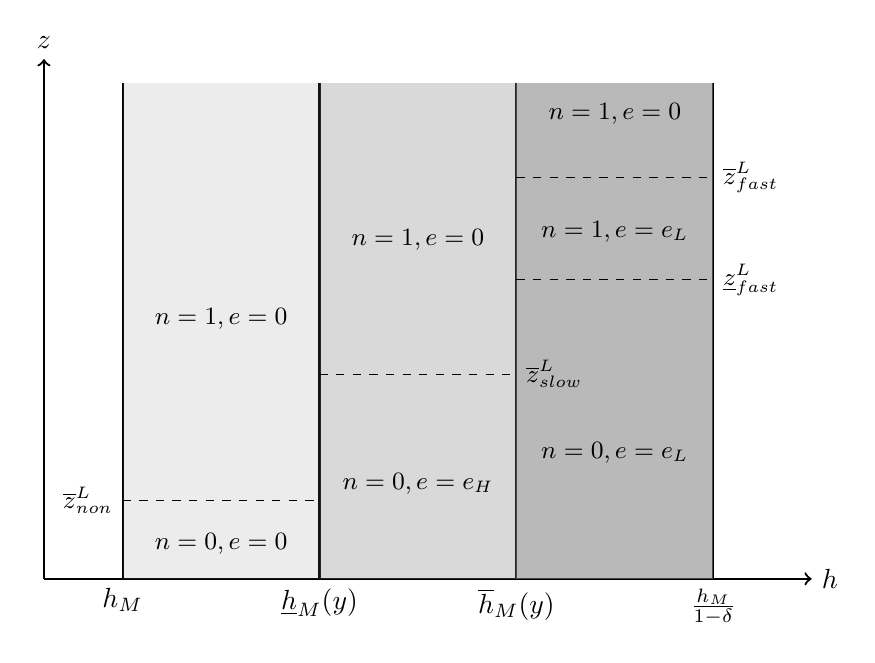
\begin{tikzpicture}[xscale=1.25]

% Decision rule conditional on a given y:
% x-axis: h in [h_M, h_M/(1-delta))
% y-axis: z

% Axes
\draw[thick,->] (-0.8,0) -- (7,0) node[right] {$h$};
\draw[thick,->] (-0.8,0) -- (-0.8,6.6) node[above] {$z$};

% h-range boundaries
\draw[thick] (0,0) -- (0,6.3);
\node[below] at (0,0) {$h_M$};
\draw[thick] (6,0) -- (6,6.3);
\node[below] at (6,0) {$\frac{h_M}{1-\delta}$};


% Learner-type cutoffs in h conditional on y (schematic placement)
\draw[thick] (2,0) -- (2,6.3);
\draw[thick] (4,0) -- (4,6.3);
\node[below] at (2,0) {$\underline{h}_M(y)$};
\node[below] at (4,0) {$\overline{h}_M(y)$};

% Shade learner-type regions (conditional on y)
\fill[gray, opacity=0.15] (0,0) rectangle (2,6.3); % non-learners
\fill[gray, opacity=0.30] (2,0) rectangle (4,6.3); % slow learners
\fill[gray, opacity=0.55] (4,0) rectangle (6,6.3); % fast learners

% z cutoffs (schematic heights)
\def\zNon{1.0}
\def\zSlow{2.6}
\def\zFastL{3.8}
\def\zFastU{5.1}

% Non-learner cutoff
\draw[dashed] (0,\zNon) -- (2,\zNon);
\node[left] at (0,\zNon) {\small $\overline{z}^L_{non}$};

% Slow-learner cutoff
\draw[dashed] (2,\zSlow) -- (4,\zSlow);
\node[right] at (4,\zSlow) {\small $\overline{z}^L_{slow}$};

% Fast-learner cutoffs
\draw[dashed] (4,\zFastL) -- (6,\zFastL);
\draw[dashed] (4,\zFastU) -- (6,\zFastU);
\node[right] at (6,\zFastL) {\small $\underline{z}^L_{fast}$};
\node[right] at (6,\zFastU) {\small $\overline{z}^L_{fast}$};

% Decision labels inside regions
% Non-learners
\node at (1,0.45) {\small $n=0,e=0$};
\node at (1,3.3) {\small $n=1,e=0$};

% Slow learners
\node at (3,1.2) {\small $n=0,e=e_H$};
\node at (3,4.3) {\small $n=1,e=0$};

% Fast learners
\node at (5,1.6) {\small $n=0,e=e_L$};
\node at (5,4.4) {\small $n=1,e=e_L$};
\node at (5,5.9) {\small $n=1,e=0$};

\end{tikzpicture}

\end{document}

\caption{Decision Rule Diagram for $h_M \leq h<h_M(1-\delta)^{-1}$}
\begin{flushleft}
\footnotesize{The human capital $h$ changes along the horizontal line and the idiosyncratic productivity $z$ changes along the vertical line. The two diagonal lines, $\overline{z}_M(h)$ and $\underline{z}_M(h)$, separate the state space into three areas: the unshaded area represents the non-learners, the lightly-shaded area represents the slow learners, and the darkly-shaded  area represents the fast learners. The areas are divided by four dashed horizontal lines associated with cutoffs $\overline{z}^L_{non}$, $\overline{z}^L_{slow}$, $\underline{z}^L_{fast}$, and $\overline{z}^L_{fast}$ that are functions of capital holding $a$.} 
\end{flushleft}
    
\label{fig:rule-diagram}
\end{figure}

\paragraph{Decision rule diagram:}Figure \ref{fig:rule-diagram} illustrates the decision rule $(n,e)$ as a function of states $(z,h,a)$ for households with $h_M \leq h<h_M\frac{1}{1-\delta}$. The human capital $h$ changes along the horizontal line and the idiosyncratic productivity $z$ changes along the vertical line. The two diagonal lines, $\overline{z}_M(h)$ and $\underline{z}_M(h)$ defined in (\ref{eq:zm}), separate the state space into three areas: the unshaded area represents the non-learners, the lightly-shaded area represents the slow learners, and the darkly-shaded area represents the fast learners. The areas are divided by four dashed horizontal lines associated with cutoffs $\overline{z}^L_{non}(a)$, $\overline{z}^L_{slow}(a)$, $\underline{z}^L_{fast}(a)$, and $\overline{z}^L_{fast}(a)$ that are functions of capital holding $a$ and defined in (\ref{eq:z-non}), (\ref{eq:z-slow}), (\ref{eq:z-fast-lower}), and (\ref{eq:z-fast-upper}).


This decision rule diagram is representative for households in other four ranges of human capital. Figure \ref{fig:e-digram} illustrates the regions in which households make positive human capital investments. Striped shading highlights where investment occurs, with dark areas denoting fast learners and light areas representing slow learners. 

For households with $h<h_M$, $\overline{z}_M(h)$ and $\underline{z}_M(h)$ continue to be the boundaries that separate non-learners, slow learners and fast learners, but the four cutoffs are $\overline{z}^L_{non}\frac{1}{1-\lambda}$, $\overline{z}^L_{slow}\frac{1}{1-\lambda}$, $\underline{z}^L_{fast}\frac{1}{1-\lambda}$, and $\overline{z}^L_{fast}\frac{1}{1-\lambda}$.

For households with $h_M\frac{1}{1-\delta} \leq h<h_H\frac{1}{1-\delta}$, the boundaries for state space division change to $\overline{z}_H(h)$ and $\underline{z}_H(h)$:
\begin{equation}\label{eq:zh}
    \underline{z}_H(h):=\frac{h_H-(1-\delta)h}{e_H}; \qquad \overline{z}_H(h):=\frac{h_H-(1-\delta)h}{e_L} 
\end{equation}
If $h_M\frac{1}{1-\delta} \leq h<h_H$, the four cutoffs that partition the decision regions for households are denoted as $\overline{z}^M_{non}(a)$, $\overline{z}^M_{slow}(a)$, $\underline{z}^M_{fast}(a)$, and $\overline{z}^M_{fast}(a)$ (see Appendix~\ref{app:cutoff_formulae} for the explicit formulae).\footnote{Appendix~\ref{app:cutoff_ranking} provides parameter restrictions for $\overline{z}^M_{fast}(a)>\underline{z}^M_{fast}(a)$.}
If $h_H \leq h<h_H\frac{1}{1-\delta}$, the analogous cutoffs are given by $\overline{z}^M_{non}\frac{1}{1+\lambda}$, $\overline{z}^M_{slow}\frac{1}{1+\lambda}$, $\underline{z}^M_{fast}\frac{1}{1+\lambda}$, and $\overline{z}^M_{fast}\frac{1}{1+\lambda}$.


Households with $h \geq h_H\frac{1}{1-\delta}$ are always non-learners, since their human capital guarantees high-sector employment next period without further investment. For them, only the cutoff $\overline{z}^H_{non}(a)\frac{1}{1+\lambda}$ matters.

\begin{figure}
    \centering
    
\documentclass{standalone}
\usepackage{tikz}
\usetikzlibrary{patterns}
\begin{document}
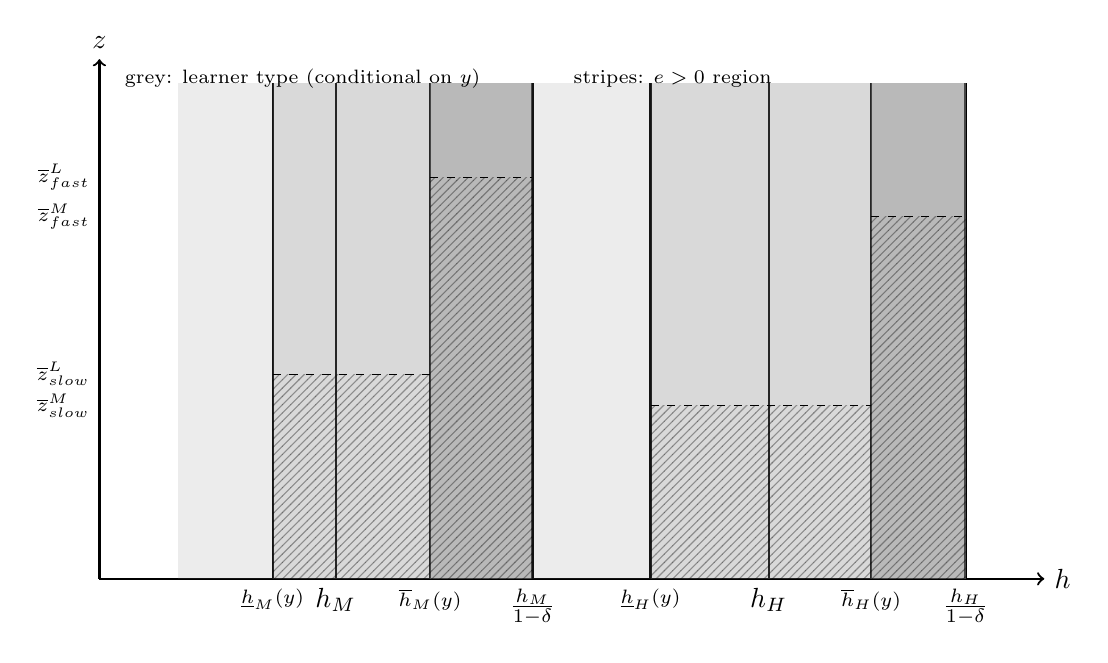
\begin{tikzpicture}

% Axes
\draw[thick,->] (-1,0) -- (11,0) node[right] {$h$};
\draw[thick,->] (-1,0) -- (-1,6.6) node[above] {$z$};

% Key h cutoffs
\draw[thick] (2,0) -- (2,6.3);
\node[below] at (2,0) {$h_M$};
\draw[thick] (4.5,0) -- (4.5,6.3);
\node[below] at (4.5,0) {$\frac{h_M}{1-\delta}$};
\draw[thick] (7.5,0) -- (7.5,6.3);
\node[below] at (7.5,0) {$h_H$};
\draw[thick] (10,0) -- (10,6.3);
\node[below] at (10,0) {$\frac{h_H}{1-\delta}$};

% h-cutoffs conditional on y (schematic placement, labels carry the economics)
% Relative to h_M
\draw[thick] (1.2,0) -- (1.2,6.3);
\draw[thick] (3.2,0) -- (3.2,6.3);
\node[below] at (1.2,0) {\scriptsize $\underline{h}_M(y)$};
\node[below] at (3.2,0) {\scriptsize $\overline{h}_M(y)$};
% Relative to h_H
\draw[thick] (6.0,0) -- (6.0,6.3);
\draw[thick] (8.8,0) -- (8.8,6.3);
\node[below] at (6.0,0) {\scriptsize $\underline{h}_H(y)$};
\node[below] at (8.8,0) {\scriptsize $\overline{h}_H(y)$};

% Grey shading: learner types (conditional on y), by h
% Left block (threshold h_M): [0,4.5]
\fill[gray, opacity=0.15] (0,0) rectangle (1.2,6.3);  % non-learners
\fill[gray, opacity=0.30] (1.2,0) rectangle (3.2,6.3); % slow learners
\fill[gray, opacity=0.55] (3.2,0) rectangle (4.5,6.3); % fast learners
% Right block (threshold h_H): [4.5,10]
\fill[gray, opacity=0.15] (4.5,0) rectangle (6.0,6.3);  % non-learners
\fill[gray, opacity=0.30] (6.0,0) rectangle (8.8,6.3);  % slow learners
\fill[gray, opacity=0.55] (8.8,0) rectangle (10,6.3);   % fast learners

% Stripes: region where e>0 (schematic, uses z cutoffs)
% Define schematic z cutoffs
\def\zSlowL{2.6}   % \overline{z}^L_{slow}
\def\zFastL{5.1}   % \overline{z}^L_{fast}
\def\zSlowM{2.2}   % \overline{z}^M_{slow}
\def\zFastM{4.6}   % \overline{z}^M_{fast}

% Left block: investment for slow learners (e_H) when z is low
\fill[pattern=north east lines, pattern color=black, opacity=0.35]
  (1.2,0) rectangle (3.2,\zSlowL);
% Left block: investment for fast learners (e_L) when z is below \overline{z}^L_{fast}
\fill[pattern=north east lines, pattern color=black, opacity=0.35]
  (3.2,0) rectangle (4.5,\zFastL);

% Right block: investment for slow learners (e_H) when z is low
\fill[pattern=north east lines, pattern color=black, opacity=0.35]
  (6.0,0) rectangle (8.8,\zSlowM);
% Right block: investment for fast learners (e_L) when z is low
\fill[pattern=north east lines, pattern color=black, opacity=0.35]
  (8.8,0) rectangle (10,\zFastM);

% Dashed horizontal cutoff lines (labels)
\draw[dashed] (1.2,\zSlowL) -- (3.2,\zSlowL);
\node[left] at (-1,\zSlowL) {\scriptsize $\overline{z}^L_{slow}$};
\draw[dashed] (3.2,\zFastL) -- (4.5,\zFastL);
\node[left] at (-1,\zFastL) {\scriptsize $\overline{z}^L_{fast}$};
\draw[dashed] (6.0,\zSlowM) -- (8.8,\zSlowM);
\node[left] at (-1,\zSlowM) {\scriptsize $\overline{z}^M_{slow}$};
\draw[dashed] (8.8,\zFastM) -- (10,\zFastM);
\node[left] at (-1,\zFastM) {\scriptsize $\overline{z}^M_{fast}$};

% Legend (minimal)
\node[anchor=west] at (-0.8,6.35) {\scriptsize grey: learner type (conditional on $y$)};
\node[anchor=west] at (4.9,6.35) {\scriptsize stripes: $e>0$ region};

\end{tikzpicture}
\end{document}


\caption{State Space for Human Capital Investment}
\begin{flushleft}
\footnotesize{The darkly-shaded striped areas indicate the state space for human capital investment equal to $e_L$ by the fast learners. The lightly-shaded striped areas indicate the state space for human capital investment equal to $e_H$ by the slow learners.} 
\end{flushleft}
    
\label{fig:e-digram}
\end{figure}





\subsection{The Effects of Uninsured Idiosyncratic Risk}
We now reintroduce the idiosyncratic risk to households in period 1 by assuming that $z'$ follows a log-normal distribution with mean $\overline{z}'$ and variance $\sigma^2_z$. 

Our previous analysis without uncertainty is a special case with $\sigma^2_z=0$. The effects of uninsured idiosyncratic risk can be thought as how households' decisions change when the distribution of $z'$ undergoes a mean-preserving spread in the sense of second-order stochastic dominance.

From a consumption-saving perspective, the uncertain $z'$ is associated with future labor income risk. It is well understood in the literature that idiosyncratic future income risk raises the expected marginal utility of future consumption for households with log utility and makes them save more. In our model, households can also supply more labor to mitigate the effect of idiosyncratic income risk on the marginal utility of consumption. 

From the perspective of human capital investment, the uncertain $z'$ is associated with risk in the return to human capital. Conditional on working, households' income increases with $z'$: $c'=(1+r')a'+w'x(h')z'$. $\ln(c')$ is increasing and concave in $z'$, and a higher $x(h')$ increases the concavity.\footnote{The marginal effect of $z'$ on $\ln(c')$ is 
\begin{equation*}
    \frac{\partial\ln(c')}{\partial z'}=\frac{w'x(h')}{(1+r')a'+w'x(h')z'} > 0
\end{equation*}
The second derivative is 
\begin{equation*}
    \frac{\partial^2\ln(c')}{(\partial z')^2}=-\left[\frac{w'x(h')}{(1+r')a'+w'x(h')z'}\right]^2 <0
\end{equation*}
and is more negative if $x(h')$ is higher.} Consider two levels of $h'$, $\overline{h'}>\underline{h'}$, a mean-preserving spread of $z'$ distribution reduces the expected utility at both levels of $h'$ but the reduction is larger for the higher level $\overline{h'}$. Hence, the expected utility gain of moving from $\underline{h'}$ to $\overline{h'}$ is smaller due to the idiosyncratic risk. Human capital investment is discouraged.

Taking into account endogenous labor supply reinforces the discouragement of human capital investment by the idiosyncratic risk. Recall from Section \ref{sec:period2} that households with $z'$ lower than a cutoff do not work. The endogenous labor supply therefore provides insurance against the lower tail risk of the idiosyncratic $z'$. Moreover, the cutoff in $z'$ is lower for those with higher human capital $h'$. This makes households with higher $h'$ more exposed to the lower tail risk than those with lower $h'$, further reducing the gain of human capital investment.


\begin{proposition}
    The uninsured idiosyncratic risk in $z'$ makes households in period 1 save more, work more and invest less in human capital.
\end{proposition}


\subsection{Period-1 Saving and Human Capital Investment}
In this section, we study the impact of endogenous human capital investment on households’ saving decisions. Specifically, we compare optimal saving behavior in two scenarios: one in which households can choose to invest in human capital, and an alternative scenario in which human capital is exogenously fixed. To facilitate the comparison, we assume in this section that there is no human capital depreciation.\footnote{If depreciation is allowed, the analysis proceeds similarly but involves more comparison paris.}

When the optimal choice of human capital investment is zero, optimal saving is identical in both scenarios. When the optimal human capital investment is either $e_L$ or $e_H$, we compare the household's optimal saving to the case where human capital investment is exogenously fixed at zero, i.e., $(n=1, e=0)$.\footnote{Why not compare to $(n=0,e=0)$? Such a comparison is not meaningful when considering $(n=1, e=e_L)$ because the two scenarios involve different state spaces. To see it, suppose conditions are 
such that $(n=1,e=e_L)$ is optimal. If we were to fix $e=0$ 
exogenously, the household’s lifetime income would fall, 
and as a result the household would have a greater 
incentive to work. Thus, it is not possible for the 
household to deviate from choosing $n=1$ when human capital 
is held fixed at $e=0$. The comparison between $(n=0,e=0)$ 
and $(n=0,e=e_L \text{ or } e_H)$ is similar to the 
comparison between $(n=1,e=0)$ to $(n=1,e=e_L)$, since human capital investment does not affect period-1 labor income in either case.}

To make the human captial relevant, we assume that $n'=1$ in period 2. The additive separability of work and human capital investment effort from consumption allows us to consider the optimal saving conditional on a given choice of labor supply and human capital investment. 

In particular, the household maximizes expected lifetime utility:   
\begin{equation}\label{eq:savingprob}
\max_{a'} : \ln(c) + \beta \mathbb{E}_{z'}[\ln(c')],
\end{equation}
subject to the budget constraints
\begin{align}
c + a' &= (1+r)a + n(wzx(h)) , \\
c' &= (1+r')a' + w'z'x(h'), \\
\text{with } h' &= ze + (1-\delta)h, e \in \{0, e_L, (1-n)e_H\}
\end{align}

\subsubsection{Effect of on-job-training on saving}\label{sec:on-job-saving}
We now compare the optimal saving between $(n=1,e=e_L)$ and $(n=1,e=0)$, where $e_L$ allows households to move to a higher sector in period 2 with higher sectoral productivity $x(h')$. 

To simplify the notation while maintaining the key economic forces, we normalize $(1+r)=(1+r')= 1$, $w=w'= 1$, the period-1 productivity shock $z=1$ and the period-2 productivity shock $z'$ to $\ln z' \sim \mathcal{N}(0,\sigma_z^2)$. The budget constraints become:
\begin{equation}
c + a' = a + x , \quad c' = a' + txz'
\end{equation}
where $t\geq 1$ represents the effect of human capital investment on period-2 income: $t>1$ if $e=e_L$; $t=1$ if $e=0$.

The optimal saving is determined by the FOC:
\begin{equation}
\frac{1}{a+x-a'} = \beta\mathbb{E}_{z'}\big(\frac{1}{a'+txz'}\big)
\end{equation}
Denoting the mean and variance of $z'$ as $\mu$ and $\Sigma$, respectively:
\begin{equation}
    \mu \equiv \mathbb{E}[z'] = e^{\sigma_z^2/2}, \quad \Sigma \equiv\operatorname{Var}(z') = e^{\sigma_z^2}(e^{\sigma_z^2}-1).
\end{equation}
The second-order approximate solution to the FOC is:
\begin{equation}
a'^*(x,a;t) = \underbrace{\frac{\beta(a+x) - tx\mu}{1+\beta}}_{\text{CE}} + \underbrace{\frac{t^2x^2\Sigma}{\beta(a+x + tx\mu)}}_{\text{Precautionary}}
\end{equation}
The first term is the \textit{certainty-equivalent} saving, which reflects the consumption smoothing motive, increasing in the period-1 resources $a+x$ and decreasing in the period-2 expected labor income $tx\mu$. The second term is the \textit{precautionary} saving, which is increasing in the variance of period-2 labor income $t^2x^2\Sigma$ and decreasing in the expected total resources $a+x+tx\mu$.

The effect of on-job-training on saving can be decomposed into two components:
\begin{equation}
    \frac{\partial a'^\star}{\partial t}(x,a;t)
    = -\frac{x\mu}{1+\beta}+\frac{x^2 \Sigma}{\beta}\frac{t\,[2(a+x) + t x \mu]}{(a+x + t x \mu)^2}.
    \label{eq:dadt_partial}
\end{equation}
The first term being negative captures the \textit{crowd-out} effect on saving via consumption-smoothing motive as on-job-training increases the expected period-2 labor income $tx\mu$. The second positive term captures the \textit{crowd-in} effect via precautionary saving motive as on-job-training exposes households to larger future income risk.

To capture the overall impact of on-job-training on saving, we define:
\begin{equation} \label{eq:dadt_integral}
    \Delta_{\text{on-job}}(x,a;t) = a'^\star(x,a;t) - a'^\star(x,a;1) = \int_1^t \frac{\partial a'^\star}{\partial u}(x,a;u) du,
\end{equation}
where $a'^\star(x,a;t)$ is the optimal saving when households undertake on-job-training, and $a'^\star(x,a;1)$ is the optimal saving when human capital is kept exogenously fixed. 

Whether on-job-training increases or decreases saving ultimately depends on the balance between the crowd-out effect (via higher expected future income) and the precautionary crowd-in effect (via heightened future income risk). The next proposition demonstrates that these effects can dominate differently depending on skill, so that the overall impact of on-job-training on saving can differ between low- and high-skilled households.



\begin{proposition}\label{prop:dadt}
    When the idiosyncratic shock is large enough, i.e., $\frac{\Sigma}{\mu}>\underline{\sigma}(t)$, on-job-training crowds out saving for low-skilled households and crowds in saving for high-skilled households: 
    for $x<x^\ast(a,t)$, $e=e_L$ lowers saving $\Delta_{\text{on-job}}(x,a;t)<0$; for $x>x^\ast(a,t)$, $e=e_L$ raises saving $\Delta_{\text{on-job}}(x,a;t)>0$.
\end{proposition}
\begin{proof}
    See Appendix~\ref{appsec: proofs}.
\end{proof}


\subsubsection{Effect of full-time training on saving}
We next compare the optimal saving between $(n=0,e=e_L \text{ or } e_H)$ and $(n=1,e=0)$. Note that  full-time training requires the households to give up their labor income in period 1, which is not the case for on-job-training. Following the same normalization and notation as in the previous subsection, we can write the budget constraints with full-time training and without training as:
\begin{align}
e=e_H: \quad c + a' &= a, \quad c' = a' + txz'\\
e=0: \quad c + a' &= a + x, \quad c' = a' + xz'
\end{align}
where $t>1$ captures the effect of full-time training on period-2 income. 

The second-order approximate solution to the optimization problem is:
\begin{align}
    e=e_H: \quad a'^*_{e_H}(x,a;t) &= \underbrace{\frac{\beta a - tx\mu}{1+\beta}}_{\text{CE}} + \underbrace{\frac{t^2x^2\Sigma}{\beta(a + tx\mu)}}_{\text{Precautionary}}\\
    e=0: \quad a'^*(x,a;1) &= \underbrace{\frac{\beta(a + x) - x\mu}{1+\beta}}_{\text{CE}} + \underbrace{\frac{x^2\Sigma}{\beta(a + x + x\mu)}}_{\text{Precautionary}}
\end{align}
so that the total effect of full-time training on saving is:
\begin{align}
    \Delta_{\text{full-time}}(x,a;t) &= a'^*_{e_H}(x,a;t) - a'^*(x,a;1)\\
    &= \Delta_{\text{on-job}}(x,a;t) - x\frac{\beta}{1+\beta} + \frac{t^2x^2\Sigma}{\beta}\frac{x}{(a+x+tx\mu)(a+tx\mu)}
\end{align}
Compared to the effect of on-job-training, represented by $\Delta_{\text{on-job}}(x,a;t)$ defined in \eqref{eq:dadt_integral}, full-time training introduces two additional effects on saving. First, it further reduces saving because households forgo their period-1 labor income, as reflected in the second term. Second, it increases precautionary saving, since having lower current resources leaves households less able to self-insure against idiosyncratic risk in period 2, which is captured by the third term. 
Denote the net additional effect of full-time training on saving as:
\begin{equation}\label{eq:dadt_fulltime}
    \Delta_H(x,a;t) \equiv  x\big[-\frac{\beta}{1+\beta} + \frac{\Sigma}{\beta}\frac{t^2x^2}{(a+x+tx\mu)(a+tx\mu)}\big]
\end{equation}
so that $\Delta_{\text{full-time}}(x,a;t)=\Delta_{\text{on-job}}(x,a;t)+\Delta_H(x,a;t)$. The next proposition shows that the net additional effect is negative and stronger for higher skilled households.

\begin{proposition}\label{prop:fulltime}
    When the idiosyncratic shock is not too large, i.e., $\frac{\Sigma}{\mu}<\overline{\sigma}(t)$, full-time training crowds out more saving than on-job-training, $\Delta_H(x,a;t)<0$. Moreover, the crowding-out effect is stronger for higher skilled households: $\Delta_H(x,a;t)$ is decreasing in $x$.
\end{proposition}
\begin{proof}
    See Appendix~\ref{appsec: proofs}.
\end{proof}


\subsection{The Effects of an Anticipated Period-2 AI Shock}
Suppose that an AI shock is anticipated to occur in period 2 and to increase the labor productivity for the low sector and the high sector but not the middle sector. The effect of AI shock on the sectoral productivity is captured by $\gamma$ with $0<\gamma<1$:
\begin{equation}
    \label{eq:xAI}
x(h')=\left \{ 
\begin{array}{cl}
1-\lambda + \gamma \lambda & \text{low sector if }h'<h_{M} \\ 
1 & \text{middle sector if }h_{M}<h'<h_{H} \\ 
1+\lambda + \gamma \lambda & \text{high sector if }h'>h_{H}%
\end{array}%
\right. 
\end{equation}
In other words, the AI shock increases average labor productivity, reduces the earnings premium for the middle sector, and enlarges the earnings premium for the high sector relative to the middle sector.

%\subsubsection{AI's effect on human capital investment and labor supply}

\subsubsection{Effects on human capital investment} 

The AI shock lowers the incentive to work in the middle sector in period 2. Consequently, households with $h < h_M/(1-\delta)$ reduce their human capital investment, while those with $h > h_M/(1-\delta)$ increase it. More specifically, the upper bounds that determine whether households undertake positive human capital investment -- denoted by $\overline{z}^L_{slow}$ and $\overline{z}^L_{fast}$ for $h < h_M/(1-\delta)$, and $\overline{z}^M_{slow}$ and $\overline{z}^M_{fast}$ for $h > h_M/(1-\delta)$ -- respond in opposite directions to the anticipated shock: the former decrease with $\gamma$ and the latter increase. This relationship is formalized below.

\begin{proposition}\label{prop:AI_human_capital}
An anticipated AI shock decreases human capital investment among households with $h < h_M/(1-\delta)$, but increases it among those with $h > h_M/(1-\delta)$. Specifically, $\overline{z}^L_{slow}$ and $\overline{z}^L_{fast}$ decrease with $\gamma$, while $\overline{z}^M_{slow}$ and $\overline{z}^M_{fast}$ increase with $\gamma$.
\end{proposition}
\begin{proof}
    See Appendix~\ref{appsec: proofs}.
\end{proof}

\subsubsection{Effects on labor supply} 
\paragraph{via income:} 
The AI shock raises period-2 labor income for households who will work in the low or high sector, leading to a positive income effect that reduces their labor supply in period 1. 

\paragraph{via full-time training:} Because full-time training and labor supply compete for time, the AI shock affects their tradeoff through its impact on human capital investment incentives. For $h>h_M/(1-\delta)$, where AI makes investing in additional skills more attractive, households are more likely to engage in full-time training and thus reduce period-1 labor supply. In contrast, for $h<h_M/(1-\delta)$, where the AI shock lowers the payoff to investing in skills, households shift away from full-time training and supply more labor in the first period. 


\subsubsection{Effects on saving}

The AI shock increases sectoral labor productivities for the low and high sectors in period 2, while leaving the middle sector's labor productivity unchanged. Its effect on saving can be analyzed as if we are varying the parameter $t$ in the functions $\Delta_{\text{on-job}}(x,a;t)$, defined in \eqref{eq:dadt_integral}, and $\Delta_{H}(x,a;t)$, defined in \eqref{eq:dadt_fulltime}. 

\begin{proposition}\label{prop:Delta}
    $\Delta_{\text{on-job}}(x,a;t)$ is convex in $t$. $\Delta_{H}(x,a;t)$ is increasing in $t$.
    \begin{itemize}
        \item If $\Delta_{\text{on-job}}(x,a;t)>0$ and $t>1$, $\Delta_{\text{on-job}}(x,a;t') > \Delta_{\text{on-job}}(x,a;t)$ for $t'>t>1$. 
        \item If $\Delta_{\text{on-job}}(x,a;t) > 0$ and $t<1$, $\Delta_{\text{on-job}}(x,a;t') < \Delta_{\text{on-job}}(x,a;t)$ for $1>t'>t$.
    \end{itemize}
\end{proposition}
\begin{proof}
    See Appendix~\ref{appsec: proofs}.
\end{proof}


\paragraph{Households who stay in the same sector}
For middle-sector households, the AI shock leaves both their incomes and saving unchanged.

By contrast, low-sector and high-sector households experience an increase in period-2 labor income $x'$ as a result of the AI shock. If they remain in the same sector without needing additional human capital investment or on-the-job training, their saving behavior in the absence of the AI shock can be compared to the scenario with fixed human capital. Following the AI shock, however, their situation resembles one with on-the-job training that enhances $x'$ (i.e., $t>1$). Thus, the effect of the AI shock on saving is captured by the on-the-job training impact, $\Delta_{\text{on-job}}(x,a;t)$.

As shown in Proposition \ref{prop:dadt}, $\Delta_{\text{on-job}}(x,a;t)$ has opposite signs for low-skill and high-skill households. This implies that the AI shock \textit{crowds out} saving among low-sector households, while it \textit{crowds in} saving for high-sector households.

For households who must undertake full-time training to remain in the high sector, $\Delta_{H}(x,a;t)$ captures the additional effect of such training on saving. In this case, a higher $x'$—brought about by the AI shock—corresponds to an increase in $t$, further boosting $\Delta_{H}(x,a;t)$ (Proposition \ref{prop:Delta}). Consequently, the AI shock \textit{crowds in} saving for high-sector households in this scenario as well.


\paragraph{Households who upskill} For low-sector households, saving behavior remains unchanged, as the AI shock does not affect their future productivity after upskilling.

For the middle-sector households who upskill via on-job-training, the AI shock boosts their future productivity gain from $\lambda$ to $(1+\gamma)\lambda$, which corresponds to a higher $t$ in $\Delta_{\text{on-job}}(x,a;t)$ with $t>1$. According to Proposition \ref{prop:Delta}, if the pre-shock effect of on-the-job training on saving is positive, the AI shock will \textit{raise} saving. However, if this effect is negative, the overall impact of the AI shock on saving becomes ambiguous.

For the middle-sector households who upskill via full-time training, there is an \textit{additional positive effect} of the AI shock on their saving, because a higher $x'$ increases $\Delta_{H}(x,a;t)$ (Proposition \ref{prop:Delta}).



\paragraph{Households who downskill} Downskilling, which reflects human capital depreciation, does not require any new investment in skills. For high-sector households who transition downward, the AI shock leaves their future productivity -- and thus their saving -- unchanged.

For middle-sector households who downskill to the low sector, their saving differs from the fixed human capital scenario by $\Delta_{\text{on-job}}(x,a;t)$ with $t<1$. The AI shock mitigates their future productivity loss by reducing it from $\lambda$ to $(1-\gamma)\lambda$, effectively increasing $t$ to a new value $t'<1$. According to Proposition \ref{prop:Delta}, if the pre-shock effect $\Delta_{\text{on-job}}(x,a;t)$ is positive, the AI shock will \textit{reduce} saving. If this effect is negative, however, the overall impact of the AI shock on saving is ambiguous.





\subsection{Limitations of the two-period model}
Up to this point, our analysis has focused on how AI influences household-level decisions regarding human capital investment, labor supply, and saving within the framework of a two-period model. While this provides valuable insights into individual behavioral responses, understanding the broader, economy-wide implications of AI requires moving to a more comprehensive setting -- a quantitative model with an infinite time horizon, endogenous asset accumulation, and general equilibrium feedback.

\paragraph{General equilibrium (GE) effects} When households adjust their investment in human capital, labor supply, and savings in response to AI, these changes aggregate up to affect the total supply of effective labor and capital in the economy. As these aggregates shift, they exert downward or upward pressure on the wage rate and the interest rate, feeding back into each household’s optimization problem. Thus, general equilibrium effects capture the intricate loop by which individual decisions shape, and are shaped by, the macroeconomic environment.

\paragraph{Composition effects} Endogenizing human capital investment injects dynamism into how households sort themselves among the three skill sectors. When an AI shock occurs, individuals may choose to retrain, upskill, or even move to lower-skilled work, reshaping the distribution of labor across sectors. This shifting composition changes the relative size of each sector, with significant consequences for both aggregate outcomes and the distributional effects of AI.


\section{A Quantitative Model \protect\label{sec:quant_model}}

We now solve the full dynamic model with infinite horizon, endogenous asset accumulation, and general equilibrium. 
We calibrate the model to reflect key features of the U.S. economy,
capturing reasonable household heterogeneity. 

\subsection{Calibration \protect\label{sec:calib}}

We calibrate the model to match the U.S. economy. For several preference
parameters, we adopt values commonly used in the literature. Other
parameters are calibrated to align with targeted moments. The model
operates on an annual time period. Table \ref{tbl:para} summarizes
the parameter values used in the benchmark model.

\begin{table}
\noindent{}%
\noindent\begin{minipage}[t]{1\columnwidth}%
\begin{center}
\caption{\protect\label{tbl:para}Parameters for the Calibration}

\begin{tabular}{crrll}
\toprule 
~Parameter  & Value  &  & Description  & Target or Reference\tabularnewline
\midrule 
$\beta$  & 0.91795 &  & Time discount factor  & Annual interest rate\tabularnewline
$\rho_{z}$  & 0.94  &  & Persistence of $z$ shocks  & See text\tabularnewline
$\sigma_{z}$  & 0.287  &  & Standard deviation of $z$ shocks  & Earnings Gini\tabularnewline
$\underline{a}$  & 0  &  & Borrowing limit  & See text\tabularnewline
$\chi_{n}$  & 2.47  &  & Disutility from working  & Employment rate\tabularnewline
$\chi_{e}$  & 1.48  &  & Disutility from HC effort  & See text\tabularnewline
$\overline{n}$  & 1/3  &  & Hours worked  & Average hours worked\tabularnewline
$e_{H}$  & 1/3  &  & High level of effort  & Average hours worked\tabularnewline
$e_{L}$  & 1/6  &  & Low level of effort  & See text\tabularnewline
$h_{M}$  & 0.41  &  & Human capital cutoff for M  & See text\tabularnewline
$h_{H}$  & 0.96  &  & Human capital cutoff for H  & See text\tabularnewline
$\lambda$  & 0.2  &  & Skill premium  & Income Gini\tabularnewline
$\alpha$  & 0.36  &  & Capital income share  & Standard value\tabularnewline
$\delta$  & 0.1  &  & Capital depreciation rate  & Standard value\tabularnewline
\bottomrule
\end{tabular}
\par\end{center}%
\end{minipage}
\end{table}

The time discount factor, $\beta$, is calibrated to match an annual
interest rate of 4 percent. We set $\chi_{n}$ to replicate an 80
percent employment rate. We calibrate $\chi_{e}$ to match the fact
that around 30 percent of the population invests in human capital.
The borrowing limit, $\text{\underbar{\ensuremath{a}},}$ is set to
0. 

We calibrate parameters regarding labor productivity process as follows.
We assume that $x$ follows the AR(1) process in logs: $\log z'=\rho_{z}\log z+\epsilon_{z}$,
where $\epsilon_{z}\sim N(0,\sigma_{z}^{2})$. The shock process is
discretized using the Tauchen (1986) method, resulting in a transition
probability matrix with 9 grids. The persistence parameter $\rho_{z}=0.94$
is chosen based on estimates from the literature. The standard deviation
$\sigma_{z}$, is chosen to match the earnings Gini coefficient of 0.63.

We deviate from the two-period model by assuming that the labor supply is a discrete choice between 0 and $\overline{n}=1/3$. This change only rescales the two-period model without altering the trade-off facing the households. But such rescaling facilitates the interpretation that households are deciding whether to allocate one-third of their fixed time endowment to work. The high-level human capital accumulation
effort, $e_{H}$ is assumed to equal $\overline{n}.$ The low-level
effort, $e_{L}$ is set to half of $e_{H}$. The skill premium across
sectors, $\lambda,$ is set at 0.2 to match the income Gini coefficient.
Human capital cutoffs, $h_{M}$ and $h_{H}$, are set so that the population shares in low, middle, and high sectors are, respectively, 20, 40, and 40 percent. This population distribution roughly matches the fractions of U.S. workers in 2014 who are employed in routine manual occupations (low sector), routine cognitive and non-routine manual (middle sector), and non-routine cognitive (high sector) \cite{cortes_disappearing_2017}.


On the production side, we set the capital income share, $\alpha,$ to 0.36, and the depreciation rate, $\delta,$ to 0.1.

\subsection{Key Moments: Data vs. Model}

In Table \ref{tbl:moments}, we present a comparison of
key moments between the model and the empirical data. The model does
an excellent job of replicating the 80\% employment rate observed
in the data. In this context, employment is defined as having positive
labor income in the given year, consistent with the common approach
used in the literature. According to \citet{OECD1998}, the share
of the population investing in human capital---those who are actively
engaged in skill acquisition or education---is approximately 30\%,
a figure well matched by the model\textquoteright s predictions. This
is an important metric because it reflects the model's capacity to
capture the dynamics of human capital formation, which plays a critical
role in shaping long-run earnings and income inequality. Additionally,
the model accurately captures the distribution of income and earnings,
aligning closely with observed data. This suggests that the model
effectively incorporates the key mechanisms driving labor market outcomes
and the corresponding distributional aspects of earnings. Although the model does not explicitly target the wealth Gini coefficient, it achieves a close match to the data: the empirical wealth Gini is 0.78, while the model produces a value of 0.76. This highlights the model’s ability to capture substantial wealth inequality in the economy.

\begin{table}
    \caption{\protect\label{tbl:moments}Key Moments}
    
    \begin{centering}
    \begin{tabular}{lccccrrrc}
    \hline 
    Moment  &  &  &  & Data  &  &  &  & Model\tabularnewline
    \hline 
    ~~Employment rate  &  &  &  & 0.80  &  &  &  & 0.80\tabularnewline
    ~~Human capital investment ratio  &  &  &  & 0.29  &  &  &  & 0.29\tabularnewline
    ~~Gini coefficient for wealth  &  &  &  & 0.78  &  &  &  & 0.76\tabularnewline
    ~~Gini coefficient for earnings  &  &  &  & 0.63  &  &  &  & 0.62\tabularnewline
    ~~Gini coefficient for income  &  &  &  & 0.57  &  &  &  & 0.58\tabularnewline
    \hline 
    \end{tabular}
    \par\end{centering}
    \end{table}

\subsection{Steady-state Distribution}
Table \ref{tab:SSdistribution} presents the steady-state distribution of population, employment, and assets across sectors. The population shares are calibrated to 20\%, 40\%, and 40\% by adjusting the human capital thresholds that define sectors. The shares of employment and assets are endogenously determined by households' labor supply and savings decisions. Notably, the high sector accounts for 46\% of total employment—exceeding its population share—indicating that a disproportionate number of households choose to work in that sector. Asset holdings are even more skewed: the high sector holds 68\% of total assets, while the low sector holds only 8\%.  
 
% Table generated by Excel2LaTeX from sheet 'Sheet1'
\begin{table}[htbp]
\begin{centering}
\caption{Distribution of Population, Employment and Assets}
\begin{tabular}{lccc}
\toprule 
Sectors  & \multicolumn{1}{l}{Pop. Share (\%)} & \multicolumn{1}{l}{Emp. Share (\%)} & \multicolumn{1}{l}{Assets Share (\%)}\tabularnewline
\midrule 
Low  & 20.76 & 18.58 & 8.07\tabularnewline
Middle  & 38.87 & 35.35 & 23.92\tabularnewline
High  & 40.35 & 46.07 & 68.01\tabularnewline
\bottomrule
\end{tabular}\label{tab:SSdistribution}
\par\end{centering}
{\scriptsize Note: Human capital cutoffs, $h_{H}$ and $h_{M}$, determine
the population share across sectors. Employment share and assets share
are implied by households labor supply decisions and saving decisions. }{\scriptsize\par}
\end{table}


\section{AI's Impact on Human Capital Adjustments}
\begin{figure}
    \centering  
    \caption{Steady-state Human Capital Distribution}
    \includegraphics[width=0.9\linewidth]{figure_204040calib/h_dist.pdf}
    \label{fig:hc_dist}    
    \caption{Transition Path for Human Capital Investment}
    \includegraphics[width=0.9\linewidth]{figure_204040calib/agg_HC.pdf}
    \label{fig:h_agg}
    
\end{figure}
We now introduce AI technology into the quantitative model, assuming that it will be implemented in 10 years and that households have full information about its arrival. We examine both the transition dynamics and the differences between the initial and new steady states. This framework allows us to analyze how the economy adjusts in anticipation of, and in response to, the adoption of AI.

The effect of AI on the sectorial productivity is modeled as in (\ref{eq:xAI}) with $\gamma=0.3$. That is, AI boosted the productivity of the low sector workers by 7.5\% and the productivity of the high sector workers by 5\%, leaving the middle sector intact. It captures the key idea that AI increases average labor productivity \parencites{Acemoglu2019a}, but reduces the earning premium for the middle sector, and enlarges the earning premium for the higher sector relative the middle sector. 



\subsection{Human Capital Adjustments}
Given the employment distribution in the initial steady state, AI is projected to increase the economy's labor productivity by 4\% on average, assuming households do not alter their decisions in response. However, changes in earning premiums incentivize households to adjust their human capital investments. 

\paragraph{Steady-state human capital distribution:}
Figure \ref{fig:hc_dist} illustrates how households reallocate across sectors in the new steady state relative to the initial one. The x-axis denotes the level of human capital, while the y-axis indicates the mass of households at each human capital level. The red vertical line marks the cutoff between the low and middle sectors, and the blue vertical line marks the cutoff between the middle and high sectors.

The gray shaded area shows the overlap between the two steady-state distributions. Within each sector, the distribution of households is skewed to the left, reflecting the tendency for human capital investment to be concentrated among those near the sectoral cutoffs. As shown in the decision rule diagram in Figure \ref{fig:e-digram}, some households seek to upgrade their skills, while others aim to remain in more skilled sectors. The blue shaded area highlights the mass of households who have exited the middle sector following the AI shock. The pink areas represent the additional mass of households in the new steady-state distribution, concentrated at the lower end of the low sector and the lower end of the high sector.


\paragraph{Transition path}
Figure \ref{fig:h_agg} reports the transition dynamics of aggregate human capital from the initial to the new steady state. The figure also displays its extensive margin (the share of households making positive human capital investments) and intensive margin (average human capital per household among those who invest).

As households reallocate from the middle sector to the low and high sectors, the net effect is a gradual decline in aggregate human capital along the transition path. This mirrors the steady-state change observed in Figure \ref{fig:hc_dist}, where the increased mass at the lower end of the low sector outweighs the increase in the high sector.

Additionally, human capital accumulation becomes increasingly concentrated among a smaller share of the population. The proportion of households making positive human capital investments steadily declines, ultimately stabilizing at a level 4\% lower than in the initial steady state. Meanwhile, the average human capital among those who invest rises, reaching a level 12\% higher than the initial steady state in the long run.\footnote{The only exception to those patterns occurs at period 10 when the positive effects of AI on sectoral productivity are realized.}



\subsection{Job Polarization}\label{sec:jobpolar}

An important implication of human capital adjustments to the AI shock is job polarization. 
Figure \ref{fig:tr_share} illustrate the transition paths of population shares and employment rates in each sector. Notably, the middle sector experiences a significant decline, with its population share decreasing by approximately 13\%. Additionally, employment within this sector plummets to a level 16\% lower than the initial steady state. In contrast, both the low and high sectors see increases in their population shares and employment rates. These dynamics indicate a reallocation of \emph{workers} from the middle sector to the low and high sectors following the introduction of AI.

\paragraph{Voluntary job polarization}
This worker reallocation aligns with the phenomenon of ``job polarization"\parencites{Goos2014}, where AI and automation technologies disproportionately replace tasks commonly performed by middle-skilled workers. However, our model introduces a complementary mechanism to the conventional understanding of this reallocation. Specifically, households in our model voluntarily exit the middle sector even before AI implementation by adjusting their human capital investments -- many middle-sector workers opt for non-employment to invest in skills that will better position
them for the post-AI labor market. To emphasize this key difference, our model deliberately abstracts from any direct negative effect of AI on middle-sector workers.

\paragraph{Employment flows more towards the low sector}

Another intriguing finding in our model is the more pronounced employment effect in the low sector compared to the high sector. In the new steady state, the employment rate in the low sector increases by 12\%, whereas in the high sector, it rises by only 0.5\%. This asymmetry in employment rate changes suggests an unbalanced reallocation of workers from the middle sector, with a greater flow toward the low sector.

This disparity arises from two key factors. First, AI enhances the productivity of low-sector workers by 7.5\% and high-sector workers by 5\%. However, this productivity differential alone does not fully account for the significant asymmetry. The second factor is the variation in labor supply elasticity across sectors. Compared to the high sector, the low sector exhibits higher labor supply elasticity, meaning that the same change in labor earnings triggers larger labor supply responses. This is because households in the low sector have lower consumption levels, making their marginal utility of consumption more sensitive to changes in their budget. Consequently, a greater proportion of households in the low sector are at the margin between employment and non-employment \citep{Chang2006}.


\begin{figure}
    \begin{centering}
    \caption{Sectoral Population and Employment Transition}
    \includegraphics[width=1\linewidth]{figure_204040calib/share}
    \label{fig:tr_share}
    \end{centering}\par
    {\scriptsize Note: The transition paths within each sector. The x-axis represents years, and the y-axis shows the percentage (or percentage point) deviation from the initial steady state. AI introduction is assumed to occur in period 10. “Pop. Share” denotes the population share within each sector. “Employment" is the percentage of households who are employed in each sector.}{\scriptsize\par}
\end{figure}







\section{The Aggregate and Distributional Effects of AI}
The aggregate and distributional effects of AI are shaped by both its direct impact on sectoral productivity and the endogenous response of human capital accumulation. By altering sectoral productivity, AI changes labor earnings, which in turn influences labor supply decisions and savings through income effects. Consequently, AI directly affects the supply of labor and capital, generating aggregate economic responses. Because AI’s productivity effects are heterogeneous across sectors, its impact is inherently distributional.

These sectoral differences also induce human capital adjustments, as households reallocate across sectors in response to changing incentives. This reallocation not only shifts the distribution of labor productivity and aggregate productivity, but also directly shapes distributional outcomes, as households’ relative positions in the income and asset distributions are altered by their movement across sectors.

In this section, we examine the importance of endogenous human capital adjustment in shaping both the transitional and long-run effects of AI. To do so, we compare the benchmark economy -- where households endogenously adjust their human capital -- with an alternative scenario in which households are held fixed at their initial steady-state human capital during the AI transition (“No HC model”). In both cases, households make endogenous decisions about consumption, savings, and labor supply. 

By contrasting the transition dynamics across these two economies, we can disentangle the direct and indirect effects of AI. The transition path in the No-HC-model isolates the direct impact of AI on aggregate and distributional outcomes, as it abstracts from any human capital adjustments. The difference in outcomes between the benchmark and the No-HC-model then reveals the indirect effects of AI that operate through households’ adjustments in human capital. This decomposition allows us to assess the relative importance of human capital dynamics in driving both the aggregate and distributional consequences of AI.


\subsection{Aggregate Implications}\label{sec:result}

\begin{figure}
\begin{centering}
\caption{\protect\label{fig:no_hc_1}Transition Path of Aggregate Variables:
Benchmark vs. No HC Models.}
\includegraphics[width=0.9\linewidth]{figure_204040calib/nohc_agg.pdf}
\par\end{centering}


{\scriptsize Note:  The transition paths of aggregate variables: benchmark vs. No HC models. The x-axis represents years, and the y-axis shows the percentage deviation from the initial steady state. AI introduction is assumed to occur in period 10. The No HC model is an economy in which workers maintain their initial steady-state level of human capital throughout the AI implementation until the new steady state is reached. }{\scriptsize\par}
\end{figure}

Figure \ref{fig:no_hc_1} shows the transition paths of key macroeconomic variables—output, consumption, investment, and employment—as well as factor prices, including the wage rate and capital return. The blue solid lines depict results from the benchmark model with endogenous human capital adjustment, while the black dashed lines represent the No-HC model in which human capital is held fixed.

\subsubsection{AI's direct impacts}

The No-HC-model isolates the direct effects of AI. In the long run, the introduction of AI leads to higher output, consumption, investment, and employment. However, in anticipation of AI (prior to period 10), output and investment decline, while consumption and employment remain stable.

Before the implementation of AI, sectoral productivity is unchanged; the only difference is households’ awareness of future increases in productivity in the low and high sectors beginning in period 10. This anticipation raises households’ expected lifetime income, prompting them to save less and consume more ahead of the actual productivity gains. As a result, aggregate capital stock falls, which lowers output and reduces the marginal product of labor while raising the marginal product of capital. Employment remains largely unchanged in this period, as sectoral productivity has not yet shifted.

Following the AI shock, sectoral productivity in the low and high sectors rises, boosting labor income, employment, and output in these sectors. Because productivity gains are labor-augmenting, the supply of efficient labor units rises sharply, causing wages to decline and capital returns to increase. Employment and investment both adjust to dampen these factor price changes. In the new steady state, the wage rate is slightly below its initial level, while the return to capital is marginally higher.

\subsubsection{AI's indirect impacts via endogenous human capital adjustments}

The difference between the No-HC model and the benchmark model captures the indirect effects of AI operating through endogenous human capital adjustments. Among all macroeconomic variables, this indirect effect is most pronounced for employment.

In anticipation of AI, employment declines as some households temporarily exit the labor market to invest in human capital and prepare for the post-AI economy.\footnote{Empirical studies, such as \citet{Lerch2021} and \citet{Faber2022}, support the short-term adverse effects of AI adoption on labor markets.} During this period, labor productivity remains unchanged, so the decline in employment directly translates to a reduction in output. Consistent with standard consumption-smoothing behavior, this reduction is mainly absorbed by lower investment. Meanwhile, the drop in employment mitigates the direct effects of AI on both wages and capital returns prior to the AI implementation.

After AI is introduced, employment rebounds as sectoral productivity increases. However, continued human capital investment by middle-sector households keeps employment lower than in the No-HC model, resulting in an almost neutral long-run effect of AI on employment. Despite this, output, consumption, and investment are all higher in the benchmark model because human capital adjustments reallocate more labor to the low and high sectors, thereby better capturing the productivity gains from AI.

This reallocation also reverses the steady-state comparison of factor prices: endogenous human capital adjustment transforms the negative direct effect of AI on the wage rate into a positive net effect, and the positive direct effect on capital returns into a negative net effect.


\subsection{Distributional Implications}

The findings above underscore the importance of accounting for human capital adjustments when assessing the aggregate impact of AI, as households actively adapt to a rapidly evolving labor market. When it comes to economic inequality, endogenously adjusting human capital plays an even more significant role.

Figure \ref{fig:no_hc_gini} shows the transition paths of Gini coefficients for earnings (labor income), total income (capital and labor income), consumption, wealth (asset holdings), and human capital. The black dashed lines represent results from the No-HC model, capturing the direct impact of AI without human capital adjustment. In contrast, the blue solid lines reflect the benchmark model, where human capital responds endogenously to both anticipated and realized changes in the skill premium induced by AI.

\subsubsection{Income, earnings, and consumption inequalities}
The comparison of transition paths between the No-HC model and the benchmark model reveals that endogenous human capital adjustments fundamentally alter the impact of AI on income, earnings, and consumption inequalities.

\paragraph{AI's direct impacts:} Without any human capital adjustments, AI's impact on inequalities is primarily driven by productivity gains in the low and high sectors -- 7.5\% and 5\%, respectively. As a result, there is little direct impact on income and earnings Gini coefficients in anticipation of AI before period 10. After AI is implemented, both income and earnings inequality decline: higher labor productivity raises earnings in the low sector, while wage declines in the middle sector compress the distribution. Consumption inequality remains largely unchanged throughout the transition.

\paragraph{Effects of AI-induced human capital adjustments:}
Allowing human capital to adjust endogenously, however, leads to pronounced job polarization, as shown in Section \ref{sec:jobpolar}. Households who would have qualified for middle-sector jobs now transition to either the low or high sector. Those moving to the low sector see reduced labor earnings, while those shifting to the high sector enjoy increased earnings. This polarization drives up earnings and income inequality, both before and after AI is implemented. As income disparities widen, consumption inequality also increases.



% This rise in inequality can
% be explained by the interactions among labor market dynamics, human
% capital accumulation, precautionary savings, and the differential
% impacts of AI on various sectors.

\begin{figure}
\begin{centering}
\caption{\protect\label{fig:no_hc_gini}Transition Path of Inequality Measures:
Benchmark vs. No HC Models.}
\par
\includegraphics[width=0.95\linewidth]{figure_204040calib/nohc_gini.pdf}
\par\end{centering}
{\scriptsize Note:  The transition paths of inequality measures: benchmark vs. No HC models. The x-axis represents years, and the y-axis shows the percentage deviation from the initial steady state. AI introduction is assumed to occur in period 10. The No HC model is an economy in which workers maintain their initial steady-state level of human capital throughout the AI implementation until the new steady state is reached.}{\scriptsize\par}


\end{figure}

\subsubsection{Wealth inequality} 

In stark contrast to the effects on income and earnings inequality, allowing for endogenous human capital adjustment mitigates the negative direct impact of AI on wealth inequality. While AI’s direct effect would otherwise widen disparities, human capital responses help dampen the increase in wealth inequality, underscoring the stabilizing role of human capital adjustments in the wealth distribution.

\paragraph{AI's direct impacts:} Without any human capital adjustment, AI's impact on households' saving works purely through income effect. In both the low and high sectors, households reduce their savings in anticipation of AI, expecting higher lifetime labor income. After AI is implemented at period 10, their savings increase alongside rising labor incomes. In contrast, households in the middle sector, anticipating a negative income effect from AI due to a lower wage rate, increase their savings prior to period 10. Once AI is introduced and the wage rate recovers, middle-sector households reduce their savings.

These shifts in sectoral saving patterns sharply increase wealth inequality before period 10, as low-sector households -- typically the least wealthy -- reduce their asset holdings. After AI is implemented and saving rates in the low sector recover, the wealth Gini coefficient declines from its peak and stabilizes at a level about 0.2\% higher than its initial steady state.


\paragraph{Effects of AI-induced human capital adjustments:}
Endogenous human capital responses introduce an additional channel. AI-induced changes in the skill premium motivate more households in the middle and high sectors to undertake full-time training, either to move into or remain in the high sector. This extensive margin adjustment requires these households to forgo labor income and rely on their assets to finance consumption, thus reducing their ability to accumulate additional savings during the transition. Meanwhile, low-sector households reduce their full-time investment in human capital, freeing up resources to save more. As a result, this endogenous response of human capital dampens the rise in wealth inequality that would otherwise occur, helping to stabilize the wealth distribution even as AI reshapes the labor market. 

{\color{red} I cannot really explain well why the wealth gini in the benchmark model is lower than in the No-HC-model, please help to improve this part.}






\section{Conclusion}

Recent studies on AI suggest that advancements are likely to reduce demand for junior-level positions in high-skill industries while increasing the need for roles focused on advanced decision-making and AI oversight. We demonstrate how human capital investments are expected to adapt in response to these shifts in skill demand, highlighting the importance of accounting for these human capital responses when assessing AI’s economic impact.

Our work points to several promising directions for future research on the economic impacts of AI. First, while general equilibrium effects—such as wage and capital return adjustments—have a limited role in our model, further research could examine how these effects might vary under different economic conditions or policy environments. Second, if governments implement redistribution policies to address AI-induced inequality, understanding how these policies influence human capital accumulation, and thus their effectiveness, would be valuable. Finally, our model assumes households have perfect foresight when making human capital investments. Relaxing this assumption could reveal new insights into the economic trajectory of AI advancements and offer important policy implications.

\printbibliography



\appendix
% Ensure equation numbers in the appendix are labeled by section: e.g., A.1, B.2, etc.
\renewcommand{\theequation}{\thesection.\arabic{equation}}
\makeatletter
\@addtoreset{equation}{section}
\makeatother


\section{Household Decision Rule Cutoffs}
\subsection{Additional cutoffs formulae for households}
\label{app:cutoff_formulae}
\begin{align}
    \overline{z}^M_{non}(a)&:=\frac{(\exp(\frac{\chi_n}{1+\beta})-1)
    [(1+r)a+\frac{w'z'}{1+r'}]}{w}  \label{eq:z-non-M} \\
    \overline{z}^M_{slow}(a)&:=\frac{(\exp(\frac{\chi_n-\chi_e e_H}{1
    +\beta})-1)[(1+r)a+\frac{w'z'(1+\lambda)}{1+r'}]+\lambda\frac
    {w'z'}{1+r'}}{w} \label{eq:z-slow-M} \\
    \underline{z}^M_{fast}(a)&:=\frac{(\exp(\frac{\chi_n}{1+\beta})
    -1)[(1+r)a+\frac{w'z'(1+\lambda)}{1+r'}]}{w} \label
    {eq:z-fast-lower-M} \\
    \overline{z}^M_{fast}(a)&:=\frac{\left\{\lambda\left[\exp(\frac
    {\chi_e e_L}{1+\beta})-1\right]^{-1}-1\right\}\frac{w'z'}{1+r'}-
    (1+r)a}{w}  \label{eq:z-fast-upper_M} \\
    \overline{z}^H_{non}(a)&:=\frac{(\exp(\frac{\chi_n}{1+\beta})-1)[(1+r)a+\frac{w'z'(1+\lambda)}{1+r'}]}{w}  
\end{align}

\subsection{Parameter restrictions for cutoffs ranking}
\label{app:cutoff_ranking}
To guarantee that $(n=0,e=e_H)$ dominates $(n=0,e=0)$, we need a lower bound for $\lambda$.
The slow learners prefer $(n=0,e=e_H)$ if and only if
\begin{equation*}
    (1+\beta)\ln c(n=0,e=e_H) - \chi_e e_H \geq (1+\beta)\ln c(n=0,e=0)
\end{equation*}
or equivalently:
\begin{align}
    \lambda \geq \underline{\lambda}_1&:=\frac{(1+r)a+\frac{w'z'}{1+r'}}{\frac{w'z'}{1+r'}}\left(1-\frac{1}{\exp(\frac{\chi_e e_H}{1+\beta})}\right) \text{ if } h<h_M\frac{1}{1-\delta} \label{app:lambda1} \\
    \lambda \geq \underline{\lambda}_3&:=\frac{(1+r)a+\frac{w'z'}{1+r'}}{\frac{w'z'}{1+r'}}\left(\exp(\frac{\chi_e e_H}{1+\beta})-1\right) \text{ if } h \geq h_M\frac{1}{1-\delta} \label{app:lambda3} 
\end{align}
    

\bigskip
\noindent
To avoid $(n=1,e=e_L)$ from being a dominated choice, we need another lower bound for $\lambda$.
To see it, recall that $(n=1,e=0)$ is better than $(n=1,e=e_L)$ if $z>\overline{z}_{fast}$, and $(n=1,e=e_L)$ is better than $(n=0,e=e_L)$ if $z>\underline{z}_{fast}$. $(n=1,e=e_L)$ is therefore the best choice over the interval $(\underline{z}_{fast},\overline{z}_{fast})$. For such an interval to exist, it must be the case that when $z=\underline{z}_{fast}$, $z<\overline{z}_{fast}$. $z=\underline{z}_{fast}$ means that the fast learners are indifferent between $(n=1,e=e_L)$ and $(n=0,e=e_L)$ so that
\begin{align}
    (1+r)a+wzx(h)+\frac{w'z'}{1+r'}&=\exp(\frac{\chi_n}{1+\beta})\left[(1+r)a+\frac{w'z'}{1+r'}\right] \text{ if } h<h_M\frac{1}{1-\delta} \\
    (1+r)a+wzx(h)+\frac{w'z'(1+\lambda)}{1+r'}&=\exp(\frac{\chi_n}{1+\beta})\left[(1+r)a+\frac{w'z'(1+\lambda)}{1+r'}\right] \text{ if } h \geq h_M\frac{1}{1-\delta} 
\end{align}
For the fast learners to prefer $(n=1,e=e_L)$ over $(n=1,e=0)$, we need
\begin{equation}\label{app:eL}
    (1+\beta)\ln\frac{c(n=1,e=e_L)}{c(n=1,e=0)} \geq \chi_e e_L
\end{equation}
If $h<h_M\frac{1}{1-\delta}$, inequality (\ref{app:eL}) is:
\begin{equation*}
    (1+\beta)\ln\frac{(1+r)a+wzx(h)+\frac{w'z'}{1+r'}}{(1+r)a+wzx(h)+\frac{w'z'(1-\lambda)}{1+r'}} \geq \chi_e e_L 
\end{equation*}
Evaluating the left-hand-side at $z=\underline{z}_{fast}$ yields:
\begin{equation}
    \lambda \geq \underline{\lambda}_2:=\frac{(1+r)a+\frac{w'z'}{1+r'}}{\frac{w'z'}{1+r'}}\left(1-\frac{1}{\exp(\frac{\chi_e e_L}{1+\beta})}\right)\exp(\frac{\chi_n}{1+\beta}) \label{app:lambda2}
\end{equation}

\noindent If $h>h_M\frac{1}{1-\delta}$, inequality (\ref{app:eL}) is:
\begin{equation*}
    (1+\beta)\ln\frac{(1+r)a+wzx(h)+\frac{w'z'(1+\lambda)}{1+r'}}{(1+r)a+wzx(h)+\frac{w'z'}{1+r'}} \geq \chi_e e_L 
\end{equation*}
Evaluating the left-hand-side at $z=\underline{z}_{fast}$ yields:
\begin{equation}
    \lambda \geq \underline{\lambda}_4:=\frac{(1+r)a+\frac{w'z'}{1+r'}}{\frac{w'z'}{1+r'}}\frac{\left(\exp(\frac{\chi_e e_L}{1+\beta})-1\right)\exp(\frac{\chi_n}{1+\beta})}{\exp(\frac{\chi_e e_L}{1+\beta})+\exp(\frac{\chi_n}{1+\beta})-\exp(\frac{\chi_e e_L + \chi_n}{1+\beta})} \label{app:lambda4}
\end{equation}

We have that $\underline{\lambda}_1>\underline{\lambda}_2$ and $\underline{\lambda}_3>\underline{\lambda}_4$ if 
\begin{equation} \label{app:eH}
    \exp(\frac{\chi_e e_H}{1+\beta})>\frac{\exp(\frac{\chi_e e_L}{1+\beta})}{\exp(\frac{\chi_e e_L}{1+\beta})+\exp(\frac{\chi_n}{1+\beta})-\exp(\frac{\chi_e e_L + \chi_n}{1+\beta})}
\end{equation}
Therefore, the inequality above implies that the conditions (\ref{app:lambda1}) and (\ref{app:lambda3}) are sufficient for the conditions (\ref{app:lambda2}) and (\ref{app:lambda4}). Furthermore, $\lambda_3 \geq \lambda_1$ so that the condition (\ref{app:lambda3}) is sufficient for the condition (\ref{app:lambda1}). 

We can then conclude that the conditions (\ref{app:lambda3}) and (\ref{app:eH}) are sufficient for 1) the slower learners always prefers $(n=0,e=e_H)$ over $(n=0,e=0)$, and 2) $\overline{z}_{fast}>\underline{z}_{fast}$, i.e., there exists state space where $(n=1,e=e_L)$ is optimal.

\subsection{Other cutoffs ranking for the two-period Model}
For the fast learners, their cutoffs rank as follows 
\begin{align}
    \frac{\overline{z}^L_{fast}(a)}{1-\lambda}&>\overline{z}^L_{fast}(a)>\overline{z}^M_{fast}(a)>\frac{\overline{z}^M_{fast}(a)}{1+\lambda}  \\
    \frac{\underline{z}^L_{fast}(a)}{1-\lambda}&>\underline{z}^M_{fast}(a)>\underline{z}^L_{fast}(a)>\frac{\underline{z}^M_{fast}(a)}{1+\lambda}
\end{align}
For the slow learners, the rank of their cutoffs is
\begin{equation}
    \frac{\overline{z}^L_{slow}(a)}{1-\lambda}>\overline{z}^M_{slow}(a)>\overline{z}^L_{slow}(a)>\frac{\overline{z}^M_{slow}(a)}{1+\lambda}
\end{equation}
For the non-learners, the rank of their cutoffs is
\begin{align}
\frac{\overline{z}^L_{non}(a)}{1-\lambda} > \overline{z}^M_{non}(a) & > \frac{\overline{z}^H_{non}(a)}{1+\lambda} > \frac{\overline{z}^M_{non}(a)}{1+\lambda}\\
\overline{z}^M_{non}(a) & > \overline{z}^L_{non}(a)
\end{align}

\section{Proof of Proposition} \label{appsec: proofs}
\subsection{Proof of Proposition \ref{prop:dadt}}
The derivative of saving with respect to $t$ is
\begin{equation}
\frac{\partial a'^\star}{\partial t}(x,a;t)
=
-\frac{x\mu}{1+\beta}
+
\frac{x^2 \Sigma}{\beta}\,
\frac{t\,[2(x+a) + t x \mu]}{\big[(x+a) + t x \mu\big]^2}.
\label{eq:dadlambda_partial}
\end{equation}

The total effect of on-job-training on saving is
\begin{equation}
    \Delta_{\text{on-job}}(x,a;t) = a'^\star(x,a;t) - a'^\star(x,a;1) = \int_1^t \frac{\partial a'^\star}{\partial u}(x,a;u) du. \label{eq:dadt_total}
\end{equation}

Define
\[
F(x,a;u)\equiv x\,\frac{u[2(x+a)+u x \mu]}{[(x+a)+u x \mu]^2}, \quad \overline{F}(x,a;t)\equiv \frac{1}{t-1}\int_1^t F(x,a;u) du.
\]
Then equation \eqref{eq:dadt_total} can be written as
\[
    \Delta_{\text{on-job}}(x,a;t)
= x(t-1)\Big[\frac{\Sigma}{\beta}\overline{F}(x,a;t)-\frac{\mu}{1+\beta}\Big].
\]

Differentiating $F(x,a;u)$ with respect to $x$ gives
\[
\frac{\partial F(x,a;u)}{\partial x}
=
\frac{2u\,a\,(a+x)}{(a+ (1+u\mu) x)^3}
>0,
\]
so $\overline{F}(x,a;t)$ is strictly increasing in $x$.

The sign of $\Delta_{\text{on-job}}(x,a;t)$ is governed by
\[
S(x,a;t)\equiv \frac{\Sigma}{\beta}\overline{F}(x,a;t)-\frac{\mu}{1+\beta}.
\]
Because $\overline{F}(x,a;t)$ is strictly increasing, $S(x,a;t)$ increases monotonically with $x$. 

For $x\to 0$, $F(x,a;u)\to 0$ and $\overline{F}(x,a;t) \to 0$ so that $S(x,a;t)\to - \frac{\mu}{1+\beta}<0$, implying $\Delta_{\text{on-job}}(x,a;t)<0$ for small $x$.

For $x\to \infty$, $F(x,a;u)\to \frac{u(2+u\mu)}{(1+u\mu)^2}$ and $\overline{F}(x,a;t) \to \overline{F}_\infty(t)\equiv \frac{1}{t-1}\int_1^t \frac{u(2+u\mu)}{(1+u\mu)^2} du$. If 
\begin{equation}
\frac{\Sigma}{\mu} > \underline{\sigma}(t) \equiv \frac{\beta}{1+\beta}\frac{1}{\overline{F}_\infty(t)}
\label{app:Klowerbound}
\end{equation}
then $S(x,a;t)>0$ for sufficiently large $x$, and hence $\Delta_{\text{on-job}}(x,a;t)>0$.

If idiosyncratic risk is large enough, i.e., condition (\ref{app:Klowerbound}) is satisfied, there exists a unique threshold $x^\ast(t)$ at which the sign flips:
\[
    \Delta_{\text{on-job}}(x,a;t)<0\ \text{for }x<x^\ast(a,t),
\qquad
\Delta_{\text{on-job}}(x,a;t)>0\ \text{for }x>x^\ast(a,t).
\]




\subsection{Proof of Proposition \ref{prop:fulltime}}

Denote 
\[
G(x,a;t)\equiv \frac{t^2x^2}{(a+x+tx\mu)(a+tx\mu)}
\]
the net additional effect of full-time training on saving can be rewritten as 
\[
\Delta_H(x,a;t) \equiv  x\big[-\frac{\beta}{1+\beta} + \frac{\Sigma}{\beta}G(x,a;t)\big]
\]

Differentiating $G(x,a;t)$ with respect to $x$ gives
\[
\frac{\partial G(x,a;t)}{\partial x}
=
\frac{t^2xa(2tx\mu+2a+x)}{(a+ tx\mu)^2(a+x+tx\mu)^2}
>0,
\]
so $G(x,a;t)$ is strictly increasing in $x$.

The limits of $G(x,a;t)$ are:
\[
G(x,a;t) \to 0 \quad (x\to 0),
\]
\[
G(x,a;t) \to G_\infty(t)\equiv \frac{t}{\mu(1+t\mu)} \quad (x\to \infty),
\]
Therefore, $G(x,a;t)<G_\infty(t)$ for any $x$.

If 
\begin{equation} \label{app:Ginfty}
    \frac{\Sigma}{\beta}G_\infty(t)<\frac{\beta}{1+\beta}, \text{ i.e. } \frac{\Sigma}{\mu} < \overline{\sigma}(t) \equiv \frac{\beta^2}{1+\beta}(\frac{1}{t}+\mu).
\end{equation}
Then $\Delta_H(x,a;t)<x[-\frac{\beta}{1+\beta}+\frac{\Sigma}{\beta}G_\infty(t)]<0$ for any $x$.

Furthermore, with some tedious algebra, we can show that for any $x$
\[
G(x,a;t)+x\frac{\partial G(x,a;t)}{\partial x}<G_\infty(t)
\]
Hence, the inequality (\ref{app:Ginfty}) also implies that
\begin{equation} 
    \frac{\partial \Delta_H(x,a;t)}{\partial x} = \frac{\Sigma}{\beta}[G(x,a;t)+x\frac{\partial G(x,a;t)}{\partial x}] - \frac{\beta}{1+\beta} < \frac{\Sigma}{\beta} G_\infty(t) - \frac{\beta}{1+\beta} < 0.
\end{equation}

\subsection{Proof of Proposition \ref{prop:AI_human_capital}}
The relevant upper bounds of $z$ for positive human capital investment are functions of $\gamma$ (to the first order approximation):
\begin{align*}
    \overline{z}^L_{slow}(a;\gamma)&= \overline{z}^L_{slow}(a;\gamma=0) - \gamma \lambda  \frac{w'z'}{w(1+r')}\\
    \overline{z}^L_{fast}(a;\gamma)&= \overline{z}^L_{fast}(a;\gamma=0) - \gamma \lambda \frac{w'z'}{w(1+r')}\frac{\exp(\frac{\chi_e e_L}{1+\beta})}{\exp(\frac{\chi_e e_L}{1+\beta})-1} \\
    \overline{z}^M_{slow}(a;\gamma)&=\overline{z}^M_{slow}(a;\gamma=0) + \gamma \lambda \frac{w'z'}{w(1+r')}\exp(\frac{\chi_n-\chi_e e_H}{1+\beta})\\
    \overline{z}^M_{fast}(a;\gamma)&= \overline{z}^M_{fast}(a;\gamma=0) + \gamma \lambda \frac{w'z'}{w(1+r')}\frac{1}{\exp(\frac{\chi_e e_L}{1+\beta})-1}
\end{align*}
Therefore, an anticipated AI shock, $\gamma>0$ makes those with $h<h_M\frac{1}{1-\delta}$ invest less human capital and those with $h>h_M\frac{1}{1-\delta}$ invest more human capital.


\subsection{Proof of Proposition \ref{prop:Delta}}

\[
    \Delta_{\text{on-job}}(x,a;t) = a'^\star(x,a;t) - a'^\star(x,a;1) = \int_1^t \frac{\partial a'^\star}{\partial u}(x,a;u) du.
\]
differentiating with respect to $t$ gives
\[\frac{d \Delta_{\text{on-job}}(x,a;t)}{d t} = \frac{\partial a'^\star}{\partial t}(x,a;t) 
\]
Since
\begin{equation}
    \frac{\partial^2 a'^*(x,a;t)}{\partial t^2}  = \frac{\partial}{\partial t} \left( -\frac{x\mu}{1+\beta}
    +
    \frac{x^2 \Sigma}{\beta}\,
    \frac{t\,[2(x+a) + t x \mu]}{\big[(x+a) + t x \mu\big]^2} \right) = \frac{2x^2\Sigma(a+x)^2}{\beta(a +x + tx\mu)^3} > 0.
\end{equation}
The slope $\frac{\partial a'^\star}{\partial t}(x,a;t)$ is strictly increasing in $t$. Hence $\Delta_{\text{on-job}}(x,a;t)$ is convex in $t$.

\[\Delta_{H}(x,a;t) = x\big[-\frac{\beta}{1+\beta} + \frac{\Sigma}{\beta}G(x,a;t)\big] \text{ with } G(x,a;t) = \frac{t^2x^2}{(a+x+tx\mu)(a+tx\mu)}
\]
Differentiating $G(x,a;t)$ with respect to $t$ gives
\[
\frac{\partial G(x,a;t)}{\partial t}
=\frac{tx^2(2a^2+2atx\mu+2ax+\mu t x^2)}{(a+ tx\mu)^2(a+x+tx\mu)^2}
>0,
\]
so $G(x,a;t)$ is strictly increasing in $t$, and so is $\Delta_{H}(x,a;t)$.

\bigskip\noindent
We now consider the comparison between $\Delta_{\text{on-job}}(x,a;t)$ and $\Delta_{\text{on-job}}(x,a;t')$ for $t'>t$.
Given $x$ and $a$, define
\[
f(t)\equiv \frac{\partial a'^*}{\partial t}(x,a;t).
\]
so $f'(t)>0$, i.e. $f(t)$ is strictly increasing in $t$.

\subsubsection*{Case 1: $1<t<t'$}

Suppose $\Delta_{\text{on-job}}(x,a;t)>0$. Then
\[
\Delta_{\text{on-job}}(x,a;t)
=\int_{1}^{t} f(u)\,du>0.
\]
Since $f$ is increasing,
\[
f(u)\le f(t)\quad\text{for all } u\in[1,t],
\]
which implies
\[
\Delta_{\text{on-job}}(x,a;t)
=\int_{1}^{t} f(u)\,du
\le (t-1)\,f(t).
\]
Because $t>1$, the inequality $\Delta_{\text{on-job}}(x,a;t)>0$ forces $f(t)>0$.

Now for any $t'>t$,
\[
f(u)\ge f(t)>0
\quad\text{for all }u\in[t,t'],
\]
and therefore
\[
\Delta_{\text{on-job}}(x,a;t')-\Delta_{\text{on-job}}(x,a;t)
=
\int_{t}^{t'} f(u)\,du
>0.
\]

We then have that:
\begin{equation}
1<t<t', \Delta_{\text{on-job}}(x,a;t)>0
\quad\Longrightarrow\quad
\Delta_{\text{on-job}}(x,a;t')>\Delta_{\text{on-job}}(x,a;t)
\end{equation}
That is, once $\Delta_{\text{on-job}}(x,a;t)$ becomes positive for $t>1$, it is strictly increasing in $t$ thereafter.

\subsubsection*{Case 2: $t<t'<1$}

For $t<1$,
\[
\Delta_{\text{on-job}}(x,a;t)
=\int_{1}^{t} f(u)\,du
= -\int_{t}^{1} f(u)\,du.
\]

Suppose $\Delta_{\text{on-job}}(x,a;t)>0$. Then
\[
-\int_{t}^{1} f(u)\,du>0
\quad\Longrightarrow\quad
\int_{t}^{1} f(u)\,du<0.
\]
Since $f$ is increasing 
\[
f(u)\ge f(t)\quad\text{for all } u\in[t,1],
\]
which implies
\[
\int_{t}^{1} f(u)\,du
\ge (1-t)\,f(t).
\]
Because $t<1$, the inequality $\Delta_{\text{on-job}}(x,a;t)>0$ forces $f(t)<0$.

Consider 
\[
\Delta_{\text{on-job}}(x,a;t')-\Delta_{\text{on-job}}(x,a;t)
=\int_{t}^{t'} f(u)\,du
\]

If $f(u)<0$ for all $u\in[t,t']$, then $\int_{t}^{t'} f(u)\,du<0$.

If there exists some $t_s\in[t,t']$ such that $f(t_s)=0$, so $f(u)<0$ for $u<t_s$ and $f(u)>0$ for $u>t_s$. Then $f(u)>0$ for $u\in[t',1]$. Hence, 
\[
\int_{t'}^{1} f(u)\,du>0
\]
This implies that
\[\Delta_{\text{on-job}}(x,a;t')=-\int_{t'}^{1} f(u)\,du<0\]
Together with the inequality $\Delta_{\text{on-job}}(x,a;t)>0$, we have that
\[\Delta_{\text{on-job}}(x,a;t')<\Delta_{\text{on-job}}(x,a;t)\]

We then have that 
\begin{equation}
t<t'<1,\ \Delta_{\text{on-job}}(x,a;t)>0
\quad\Longrightarrow\quad
\Delta_{\text{on-job}}(x,a;t')<\Delta_{\text{on-job}}(x,a;t).
\end{equation}
Thus, for $t<1$, whenever $\Delta_{\text{on-job}}(x,a;t)>0$, increasing $t$ toward $0$ makes $\Delta_{\text{on-job}}$ strictly decrease.



\section{Computational Procedure for the Quantitative Model}

\subsection{Steady-state Equilibrium}

In the steady-state, the measure of households, $\mu(a,h,x)$, and
the factor prices are time-invariant. We find a time-invariant distribution
$\mu$. We compute the households' value functions and the decisions
rules, and the time-invariant measure of the households. We take the
following steps:
\begin{enumerate}
\item We choose the number of grid for the risk-free asset, $a,$ human
capital, $h$, and the idiosyncratic labor productivity, $x$. We
set $N_{a}=151$, $N_{h}=151$, and $N_{x}=9$ where $N$ denotes
the number of grid for each variable. To better incorporate the saving
decisions of households near the borrowing constraint, we assign more
points to the lower range of the asset and human capital. 
\item Productivity $x$ is equally distributed on the range $[-3\sigma_{x}/\sqrt{1-\rho_{x}^{2}}]$.
As shown in the paper, we construct the transition probability matrix
$\pi(x'|x)$ of the idiosyncratic labor productivity.
\item Given the values of parameters, we find the value functions for each
state $(a,h,x).$ We also obtain the decision rules: savings $a'(a,h,x)$,
and $h'(a,h,x)$. The computation steps are as follow:
\item After obtaining the value functions and the decision rules, we compute
the time-invariant distribution $\mu(a_{},h,x)$ .
\item If the variables of interest are close to the targeted values, we
have found the steady-state. If not, we choose the new parameters
and redo the above steps.
\end{enumerate}

\subsection{Transition Dynamics}

We incorporate the transition path from the status quo to the new
steady state. We describe the steps below.
\begin{enumerate}
\item We obtain the initial steady state and the new steady state.
\item We assume that the economy arrives at the new steady state at time
$T$. We set the $T$ to 100. The unit of time is a year.
\item We initialize the capital-labor ratio $\{K_{t}/L_{t}\}_{t=2}^{T-1}$
and obtain the associated factor prices $\{r_{t},w_{t}\}_{t=2}^{T-1}$. 
\item As we know the value functions at time $T$, we can obtain the value
functions and the decision rules in the transition path from $t=T-1$
to $1$. 
\item We compute the measures $\{\mu_{t}\}_{t=2}^{T}$ with the measures
at the initial steady state and the decision rules in the transition
path. 
\item We obtain the aggregate variables in the transition path with the
decision rules and the distribution measures. 
\item We compare the assumed paths of capital and the effective labor with
the updated ones. If the absolute difference between them in each
period is close enough, we obtain the converged transition path. Otherwise,
we assume new capital-labor ratio and go back to 3.
\end{enumerate}

\section{Investigating the GE channel of AI's impact}

\begin{figure}
    \centering
    \caption{Caption}
    \includegraphics[width=0.8\linewidth]{figure_204040calib/pe_agg.pdf}    
    \label{fig:placeholder}
    \caption{Caption}
    \includegraphics[width=0.8\linewidth]{figure_204040calib/pe_gini.pdf}
    \label{fig:placeholder}
\end{figure}

\paragraph{Redistribution versus general equilibrium effects:}

The effects of human capital adjustments on AI's aggregate impacts operate through two primary channels: the \textit{redistribution channel}, which reallocates households across skill sectors, and the \textit{general equilibrium (GE) channel}, which operates through changes in wages and capital returns. We now assess the relative importance of these channels in shaping economic outcomes.

Figure \ref{fig:no_hcPE_1} compares the transition dynamics between scenarios with and without human capital adjustments, while holding wages and capital returns fixed at their initial steady-state levels to eliminate GE effects. We refer to the former as the PE Model" and the latter as the "No-HC PE Model." The difference between the solid blue line and the dashed red line isolates the effect of redistribution channel. Comparing this difference to the gap between the benchmark model and the No HC model in Figure \ref{fig:no_hc_1} enables us to evaluate the importance of the redistribution channel relative to the GE channel. Two key observations emerge.

First, the \textit{redistribution channel} alone accounts for all the \textit{qualitative effects} of human capital adjustments on AI's aggregate impacts.  Redistribution of human capital increases consumption, even before AI implementation, as more households shift to the high sector. It also reduces investment by mitigating precautionary savings and lowers employment as middle-sector workers leave the labor market to invest in human capital. In the long run, redistribution amplifies AI's positive impact on output by reallocating more workers to sectors that benefit most from AI advancements.

Second, the \textit{GE channel} primarily affects the \textit{quantitative magnitude} of human capital adjustments' impact on AI's aggregate outcomes. When the GE channel is included, the differences in output, consumption, and employment between models with and without human capital adjustments are smaller compared to when the GE channel is excluded. In contrast, and somewhat unexpectedly, the difference in investment is larger when the GE channel is included. This indicates that allowing capital returns to adjust amplifies the impact of human capital accumulation on how household savings respond to AI.

When the \textit{GE channel} is active (Figure \ref{fig:no_hc__2}), AI reduces the wealth Gini, but the \textit{redistribution channel} moderates this effect. However, when the \textit{GE channel} is disabled (Figure \ref{fig:no_hcPE_2}), AI increases wealth inequality in the long run without the \textit{redistribution channel} from human capital adjustment. In contrast, with the \textit{redistribution channel} active, AI reduces wealth inequality.

These observations lead to two key conclusions:

First, the \textit{redistribution channel} alone introduces a qualitative shift in AI's long-run impact on the wealth Gini (as shown in Figure \ref{fig:no_hcPE_2}). 

Second, the \textit{GE channel}, when combined with human capital adjustment, qualitatively alters the effect of anticipating AI on the wealth Gini (as shown by comparing the blue lines in Figures \ref{fig:no_hc__2} and \ref{fig:no_hcPE_2}).

\paragraph{Policy implications:} The impact of human capital adjustments on AI's distributional outcomes, along with the roles of the \textit{redistribution channel} and \textit{GE channel}, provides valuable insights for policy discussions on how to address the challenges posed by AI shocks.

In particular, government interventions aimed at stabilizing wages in response to AI-induced economic shocks may unintentionally worsen wealth inequality. Our analysis indicates that if wages are prevented from adjusting to reflect productivity differences, this distorts households' incentives to adjust their human capital and precautionary savings—both of which play a critical role in mitigating wealth inequality.



\end{document}
